
\newif\ifcrossling\crosslingtrue
\newif\ifitmtree\itmtreetrue
\newif\iflong\longfalse
\newif\ifevaluation\evaluationfalse
\newif\ifconjugacy\conjugacyfalse
\newif\ifnonpar\nonparfalse
\newif\ifling\lingfalse
\newif\ifhighlevel\highleveltrue
\newif\iftmreview\tmreviewfalse
\newif\ifevocation\evocationfalse
\newif\ifjobtalk\jobtalktrue
\newif\ifsupershortmlslda\supershortmlsldatrue

\documentclass[compress]{beamer}

%\usepackage{beamerthemesplit}
\usepackage{xmpmulti}

\definecolor{green}{rgb}{0,.3,0}

\usepackage{graphicx,float,wrapfig, bbm}
\usepackage{amsfonts, bbold, comment}
\usepackage{mdwlist}
\usepackage{listings}
\usepackage{environ}
\usepackage{subfigure}
\usepackage{rotating}
\usepackage{algorithmic}
\usepackage{algorithm}
\usepackage{overpic}
\usepackage{qtree}
\usepackage{mathtools}

\usepackage{multirow}

\usetheme[bullet=circle,                     % Use circles instead of squares for bullets.
          titleline=true,                    % Show a line below the frame title.
          showdate=true,                     % show the date on the title page
          alternativetitlepage=true,         % Use the fancy title page.
          titlepagelogo=general_figures/culogo,              % Logo for the first page.
          % Logo for the header on first page.
          headerlogo=general_figures/boulder_cs,
          ]{UCBoulder}

\usecolortheme{ucdblack}

%\useoutertheme{infolines}
%\usetheme{Boadilla}
%\usetheme{Singapore}
% \usecolortheme{umd}
\title{Framing, Relationships, and Betrayal}
\author{Jordan Boyd-Graber}
\date{28. February 2017}


\institute[] % (optional, but mostly needed)
{University of Colorado Boulder}


\newcommand{\fsi}[2]{
\begin{frame}[plain]
\vspace*{-1pt}
\makebox[\linewidth]{\includegraphics[width=\paperwidth]{#1}}
\begin{center}
#2
\end{center}
\end{frame}
}

\newcommand{\gfxtp}[2]{
\begin{center}
	\includegraphics[width=#2\linewidth]{teaparty/figures/#1}
\end{center}
}

\newcommand{\gfxag}[2]{\begin{center}
    \includegraphics[width=#2\linewidth]{onlineag/#1}
\end{center}
}

\newcommand{\AgHeader}[1]{\multicolumn{3}{c}{\begin{small}
      #1 \end{small} } \\ \hline}
\newcommand{\AgNonTerm}[2] {\textsc{#1}$_{#2}$}
\newcommand{\AgAdNonTerm}[2] {\underline{\textsc{#1}}$_{#2}$}
\newcommand{\AgRule}[2] { #1 $\mapsto$ #2 }
\newcommand{\AgEmpty}[1] { & & #1 }
\newcommand{\AgRange}[2] {$#1 = 1, \dots, #2$}
\newcommand{\tng}[1]{\mbox{\textsc{tng}}_{#1}}

\newcommand{\subtwo}[2]{_{#1, #2}}
\newcommand{\subthree}[3]{_{#1, #2, #3}}


\newcommand{\explain}[2]{\underbrace{#2}_{\mbox{\footnotesize{#1}}}}
\newcommand{\dir}[1]{\mbox{Dir}(#1)}
\newcommand{\mult}[1]{\mbox{Mult}( #1)}
\newcommand{\Beta}[1]{\mbox{Beta}( #1)}
\newcommand{\G}[1]{\Gamma \left( \textstyle #1 \right)}
\newcommand{\LG}[1]{\log \Gamma \left( \textstyle #1 \right)}
\newcommand{\WN}[0]{\textsc{WordNet}}
\newcommand{\itmspace}[0]{\hspace{2cm}}
\newcommand{\abr}[1]{\textsc{#1}}
\newcommand{\lda}[0]{\abr{lda}}
\newcommand{\slda}[0]{\abr{slda}}

\newcommand{\digam}[1]{\Psi \left( \textstyle #1 \right) }
\newcommand{\ddigam}[1]{\Psi' \left( \textstyle #1 \right) }
\newcommand{\e}[2]{\mathbb{E}_{#1}\left[ #2 \right] }
\newcommand{\ind}[1]{\mathbb{I}\left[ #1 \right] }
\newcommand{\ex}[1]{\mbox{exp}\left\{ #1\right\} }
\newcommand{\D}[2]{\frac{\partial #1}{\partial #2}}
\newcommand{\elbo}{\mathcal{L}}


\newcommand{\citename}[1]{\emph{#1} }
\newcommand{\bm}[1]{\mbox{\boldmath$#1$}}
\newcommand{\Dir}{\mathrm{Dir}}
\newcommand{\Mult}{\mathrm{Mult}}
\newcommand{\g}[1]{\Gamma \left( #1 \right)}
\newcommand{\paragraph}[1]{ \vskip 1cm {\bf \large #1}}

\NewEnviron{smalign}{
\vspace{-.6cm}
\begin{small}
\begin{align}
  \BODY
\end{align}
\end{small}
\vspace{-.6cm}
}


\providecommand{\graphscale}{0.6}

\newcommand{\danquote}[1]{

\begin{flushright}
\begin{overpic}[width=5.5cm,tics=10]{general_figures/speech_bubble}
	\put(10,30) { \parbox{4cm}{#1 }}
\end{overpic}

\includegraphics[width=1.5cm]{general_figures/milkman_dan}
\end{flushright}
}


% \AtBeginSection[] % "Beamer, do the following at the start of every section"
% { \begin{frame}

% \frametitle{Outline} % make a frame titled "Outline"
% \tableofcontents[currentsection] % show TOC and highlight current section
% \end{frame} }

\lstset{language=Python}

\DeclareMathSymbol{\R}{\mathbin}{AMSb}{"52}

\setbeamertemplate{footline}{}

\begin{document}

% this prints title, author etc. info from above

\frame{
\titlepage
\tiny
}



\begin{frame}{What does text say about us?}

  \begin{itemize}
    \item Can the way we speak reveal our \alert<1>{political leanings}?
    \item Can we describe \alert<2>{relationships} from dialog and description?
    \item Can the way we speak reveal \alert<3>{deception}?
  \end{itemize}

  \begin{columns}
    \column{.3\linewidth}
    \gfxtp{polarization_1}{.7}
\column{.3\linewidth}
    \includegraphics[width=.9\linewidth]{relationships/gollum_frodo}
\column{.3\linewidth}
    \includegraphics[width=.9\linewidth]{diplomacy/ceasar}
    \end{columns}

\end{frame}


\frame{

\begin{columns}

\column{.5\linewidth}

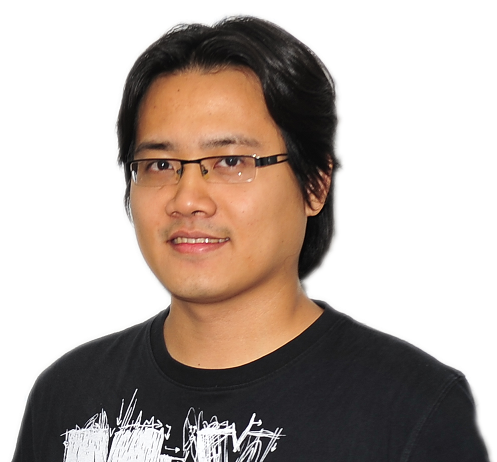
\includegraphics[width=.8\linewidth]{general_figures/an}

\column{.5\linewidth}

\begin{block}{Lexical and Hierarchical Topic Regression}
Viet-An Nguyen, Jordan Boyd-Graber, and Philip Resnik. NIPS 2013.
\end{block}

\end{columns}

}

\providecommand{\shlda}{\textsc{ShLDA}}


% The problem of framing
\begin{frame}{Message Matters}

\begin{itemize}
  \item People make radically different decisions based on how information is
  presented~\cite{tversky-92}
  \item Politicians and marketers do this too
\begin{columns}
\column{.45\linewidth}
\begin{block}{Gain frame}
    Flossing your teeth daily removes particles of food in the mouth, avoiding bacteria, which promotes great breath.
\end{block}
\column{.49\linewidth}
\begin{block}{Loss frame}
    If you do not floss your teeth daily, particles of food remain in the mouth, collecting bacteria, which causes bad breath.
\end{block}

\end{columns}
\pause
  \item Can we discover this automatically?
\end{itemize}




\end{frame}

% Our model

\begin{frame}{The data}
  \begin{columns}
    \column{.5\linewidth}
    \begin{itemize}
      \item Every document has an associated {\bf response variable}
        \begin{itemize}
      \item Politicians: \alert<1>{Ideology of speaker}
      \item Products: \alert<2>{Stars on a review}
       \end{itemize}
      \item We need the response to find association of frame and topic
    \end{itemize}

    \column{.5\linewidth}
    \only<1>{
    \begin{center}
    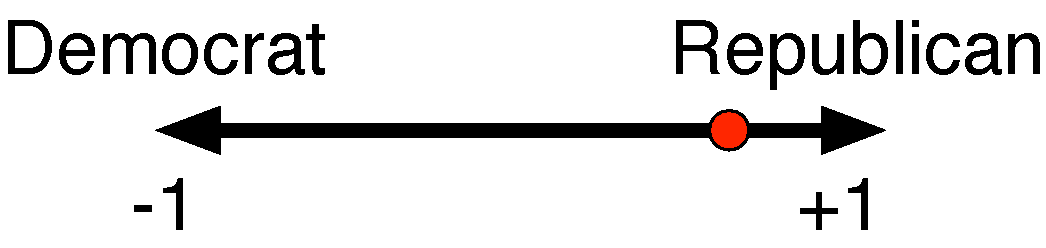
\includegraphics[width=0.8\linewidth]{shlda/ideology_scale}
    \end{center}
       \begin{block}{}
       This Christmas I want you to do the most loving thing and I want you to buy each of your children an SKS rifle and 500 rounds of ammunition.
       \end{block}
    }
    \only<2>{
      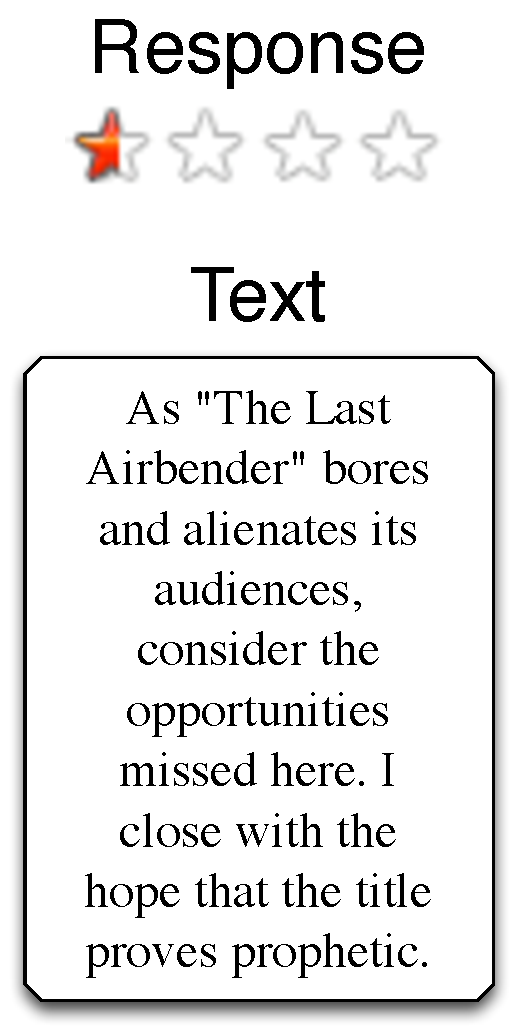
\includegraphics[width=0.6\linewidth]{shlda/response}
      }

  \end{columns}
\end{frame}

\begin{frame}{Our Model}


\providecommand{\shldascale}{0.3}

\centering
  \only<1>{ 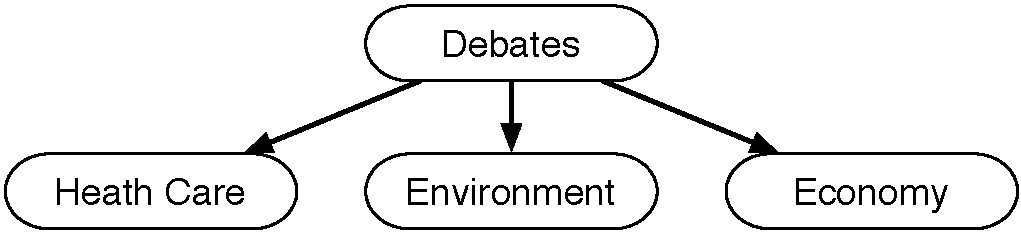
\includegraphics[scale=\shldascale]{shlda/intuition_topics_0}}
  \only<2>{ 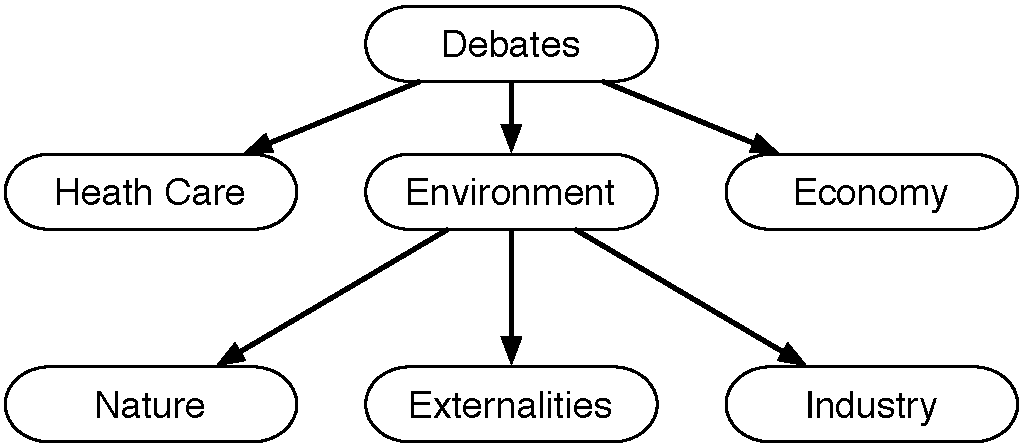
\includegraphics[scale=\shldascale]{shlda/intuition_topics_1}}
  \only<3>{ 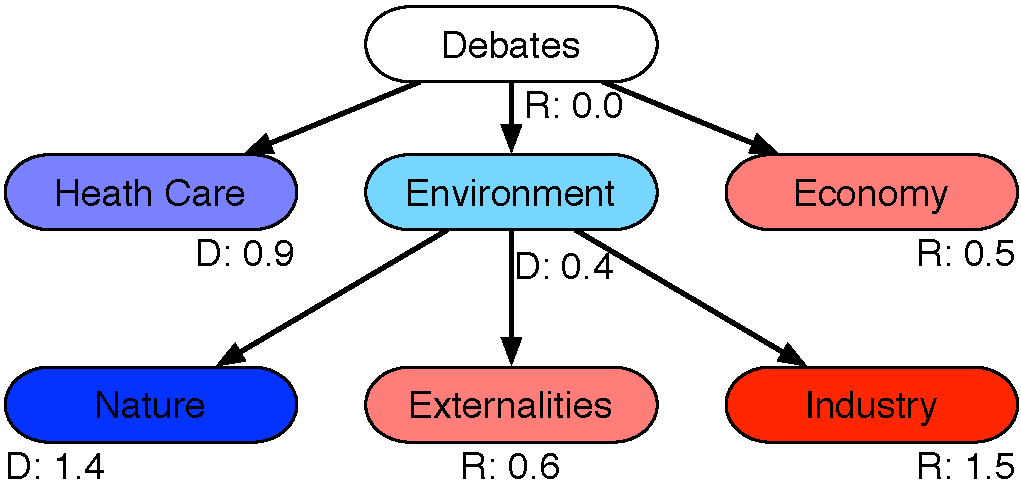
\includegraphics[scale=\shldascale]{shlda/intuition_regression_0}}
  \only<4>{ 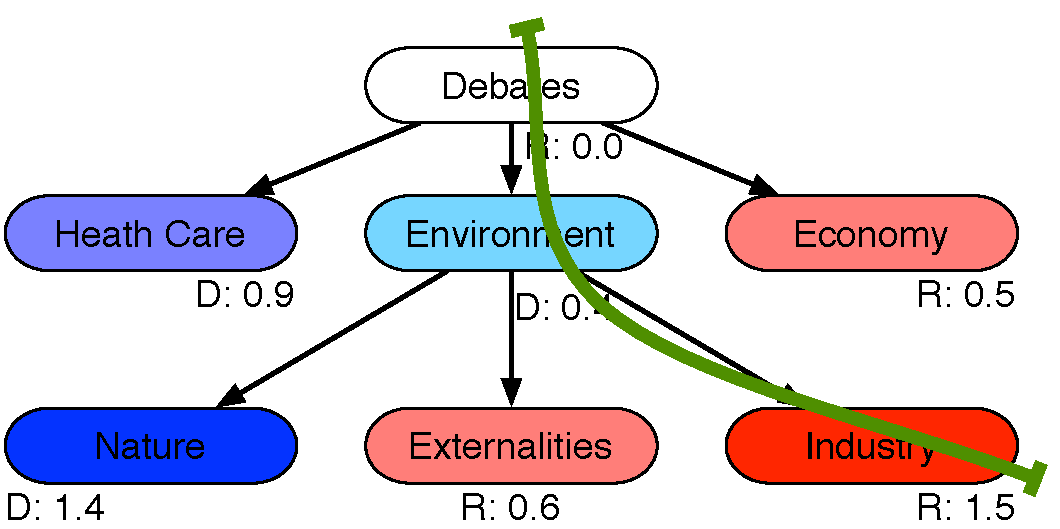
\includegraphics[scale=\shldascale]{shlda/intuition_regression_1}}
  \only<5>{ 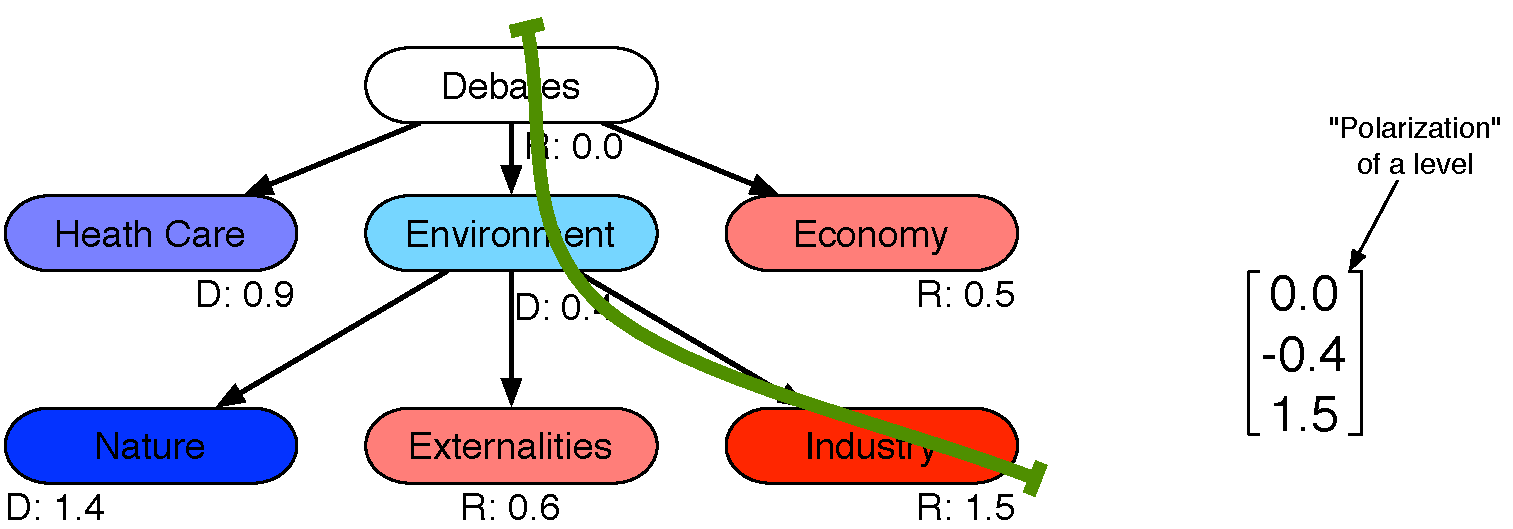
\includegraphics[scale=\shldascale]{shlda/intuition_regression_2}}
  \only<6>{ 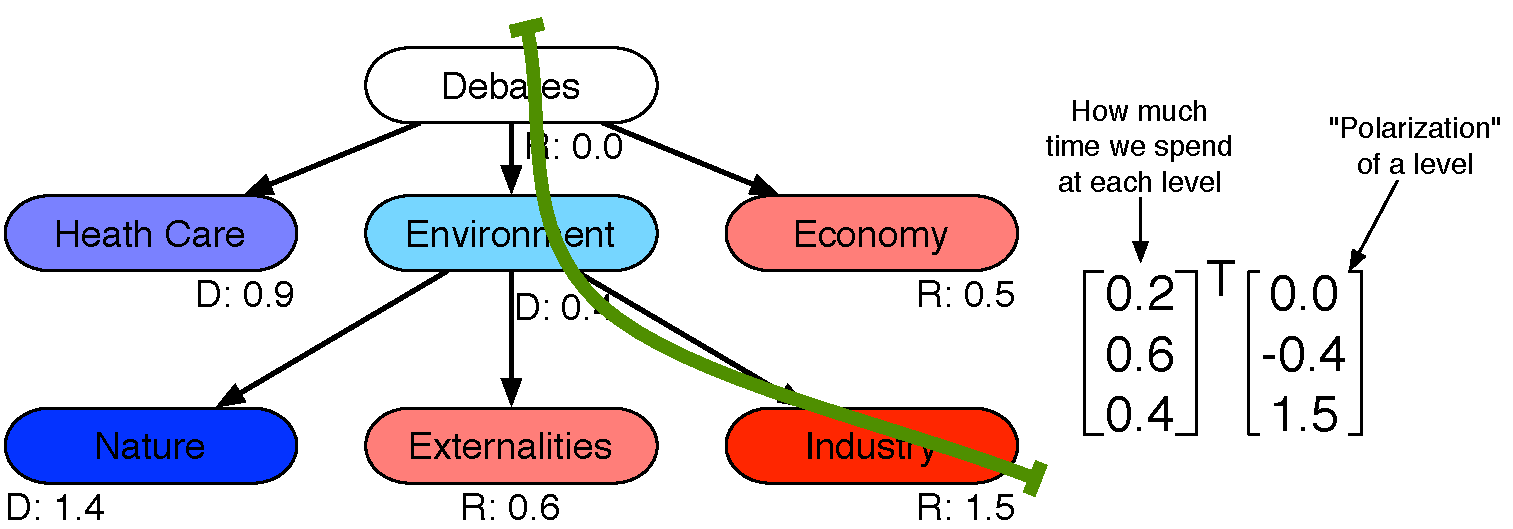
\includegraphics[scale=\shldascale]{shlda/intuition_regression_3}}
  \only<7>{ 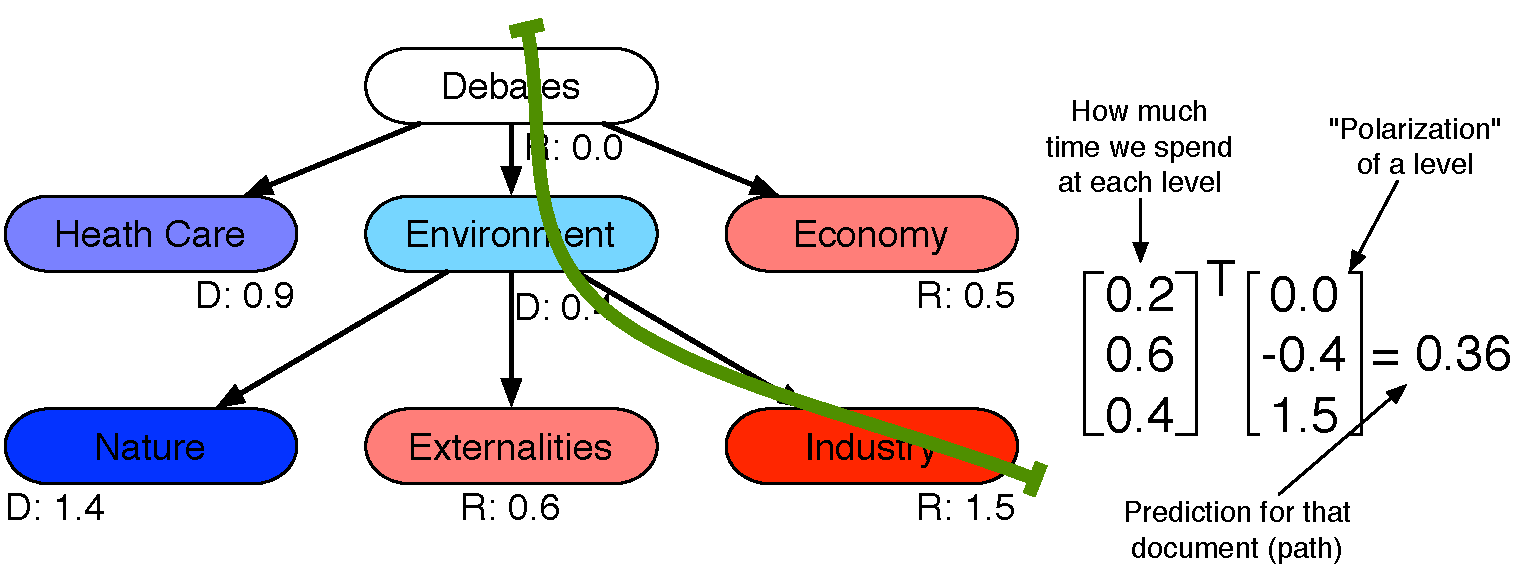
\includegraphics[scale=\shldascale]{shlda/intuition_regression_4}}
  \only<8>{ 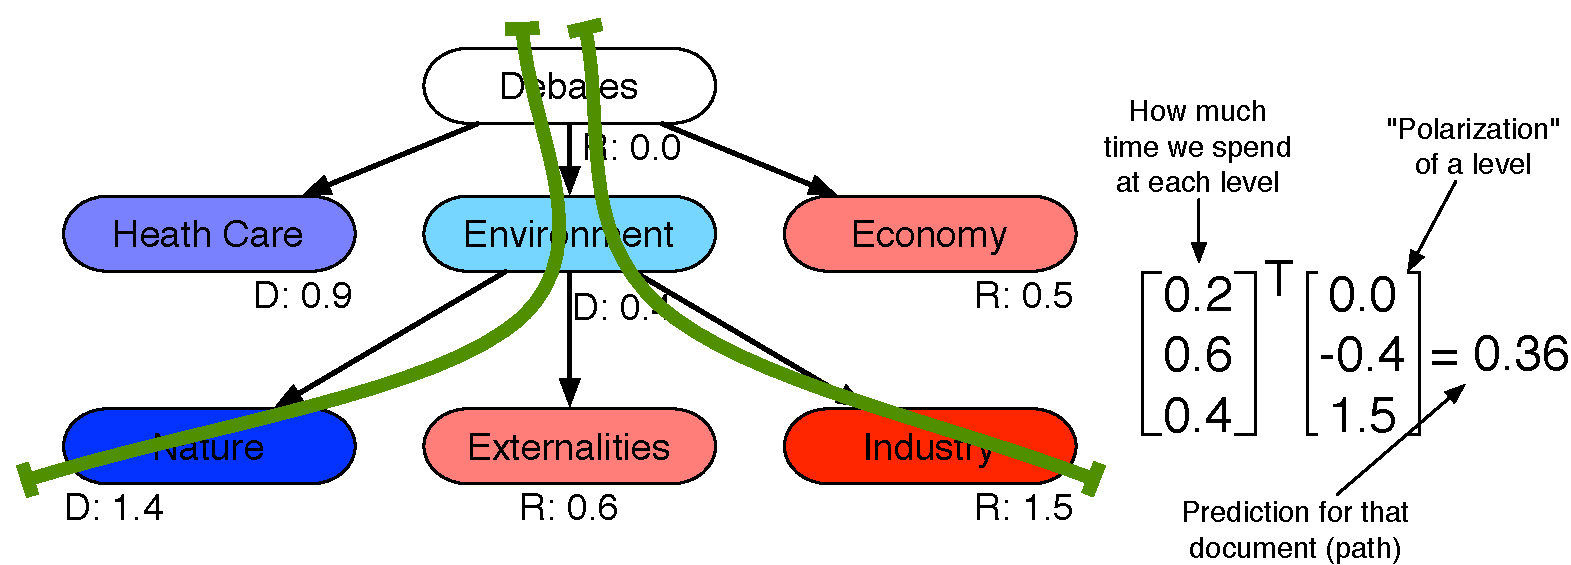
\includegraphics[scale=\shldascale]{shlda/intuition_regression_5}}
  \only<9>{ 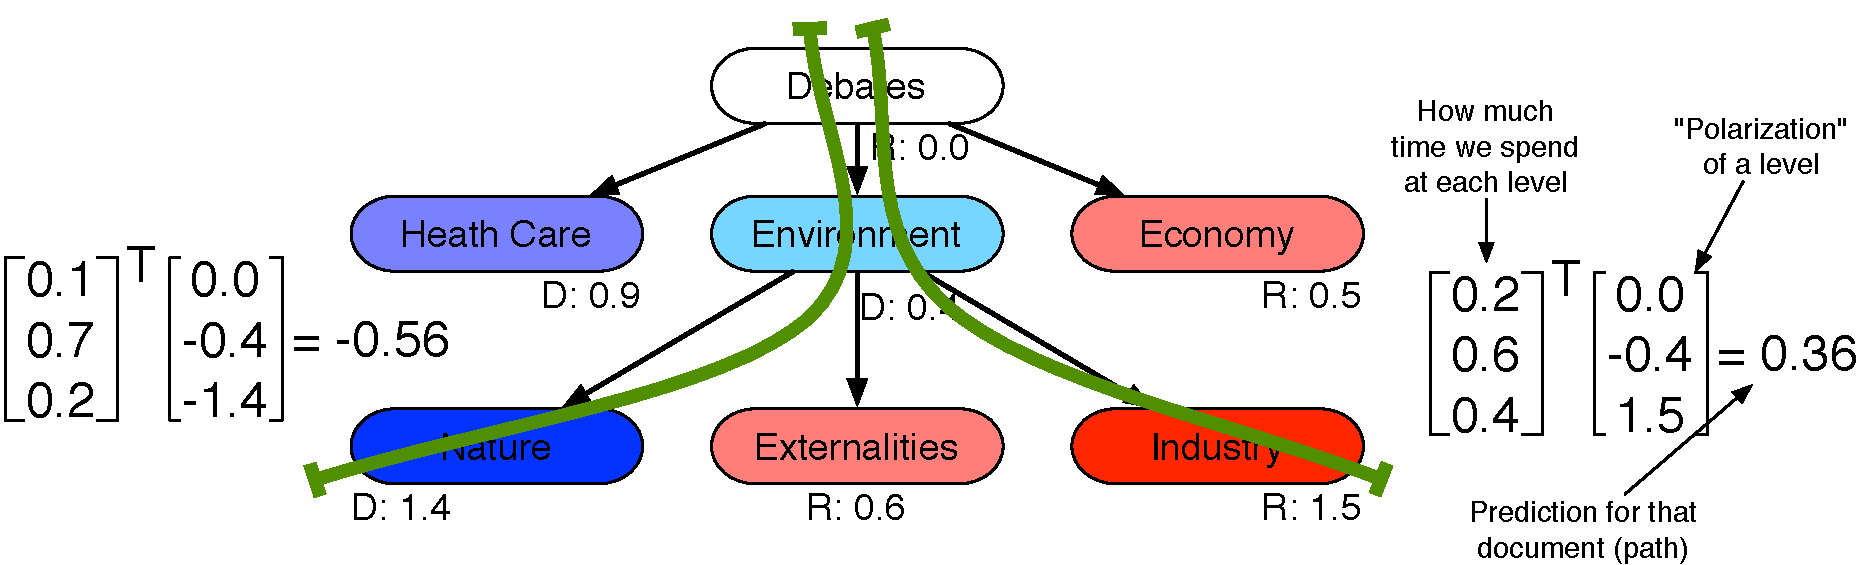
\includegraphics[scale=\shldascale]{shlda/intuition_regression_6}}
  \only<10>{ 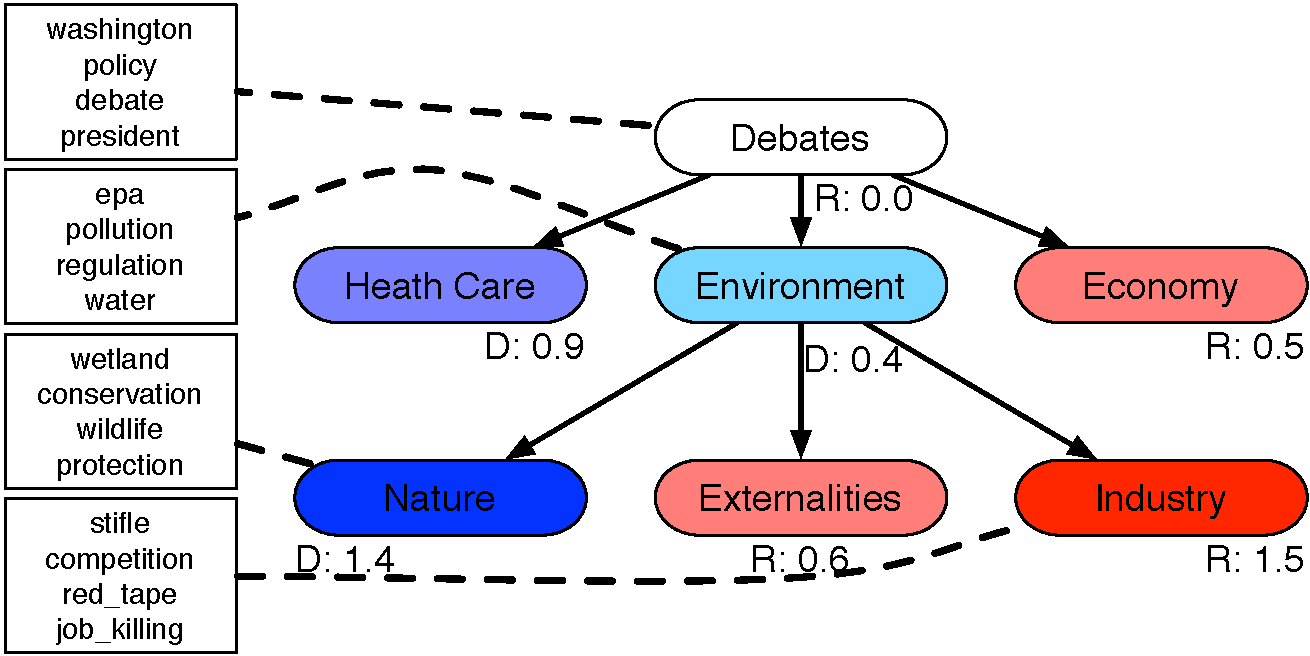
\includegraphics[scale=\shldascale]{shlda/intuition_full_0}}
  \only<11->{ 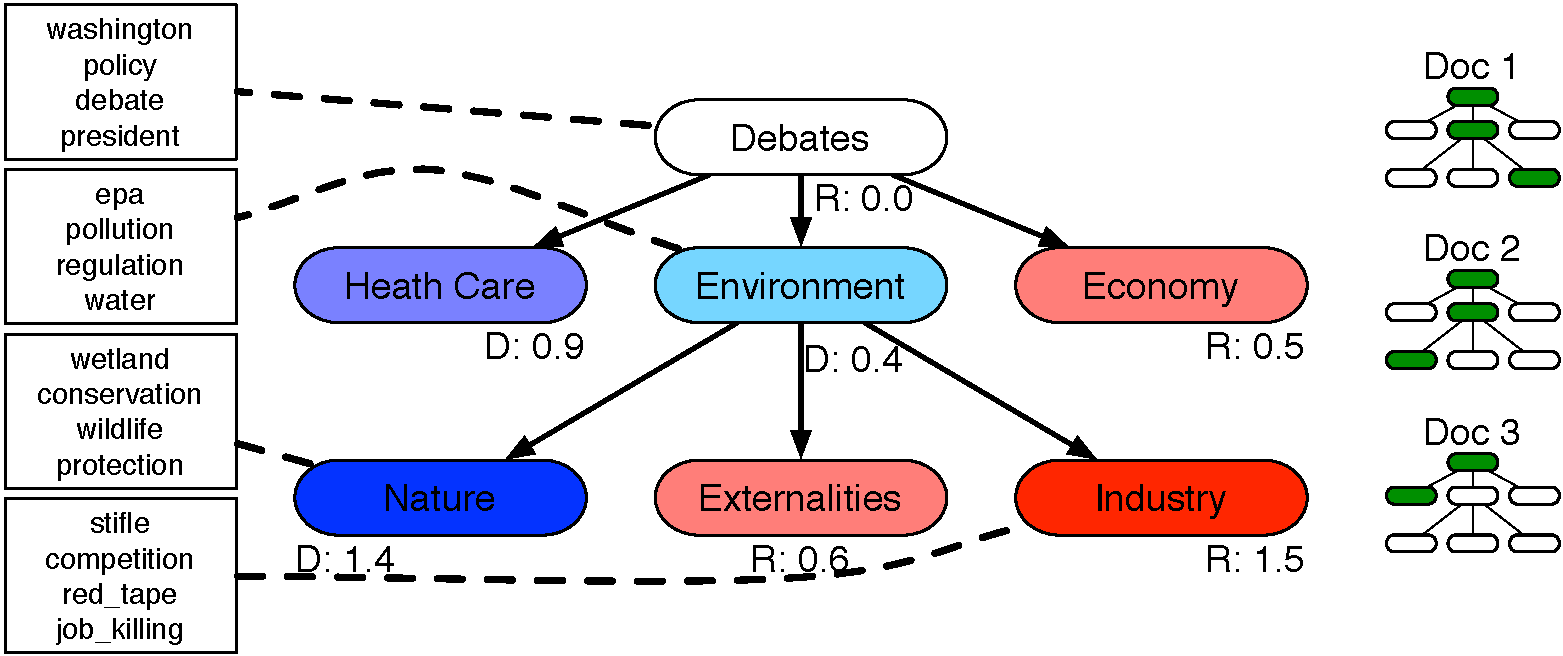
\includegraphics[scale=\shldascale]{shlda/intuition_full_1}}

  \only<11->{We call this model \alert<14>{supervised} \alert<13>{hierarchical} \alert<12>{latent Dirichlet
    allocation} (SHLDA).}

\end{frame}

% Examples


\begin{frame}{Adding in Lexical Regression}

\centering
    \only<1>{ 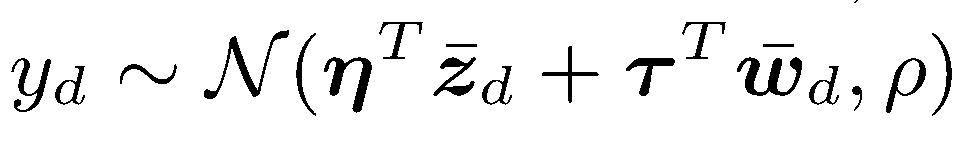
\includegraphics[width=.6\linewidth]{shlda/equation_0}}
    \only<2>{ 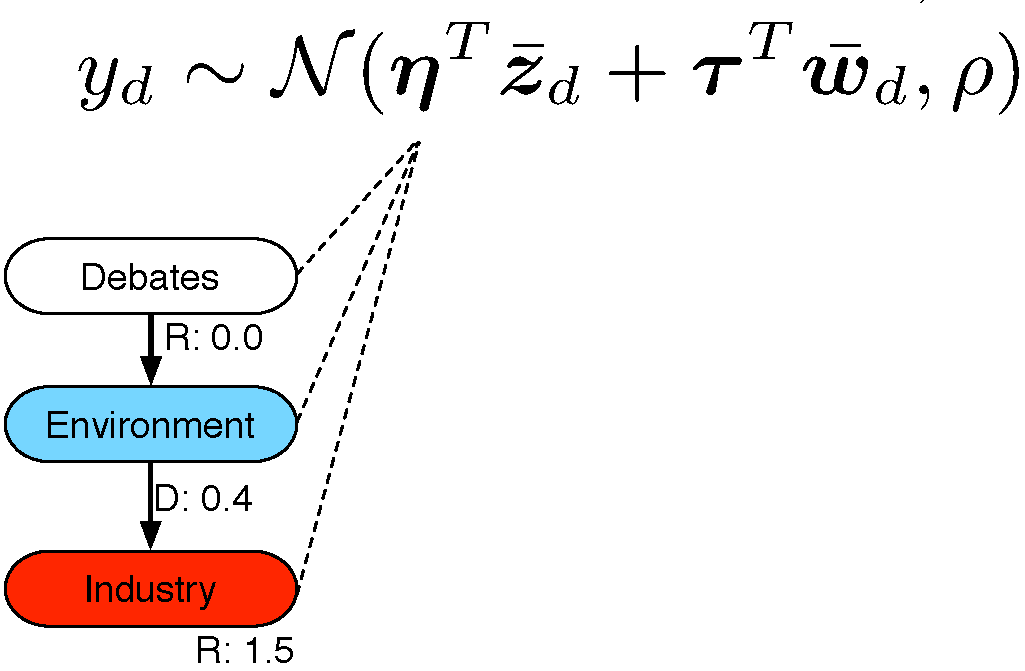
\includegraphics[width=.65\linewidth]{shlda/equation_1}}
    \only<3>{ 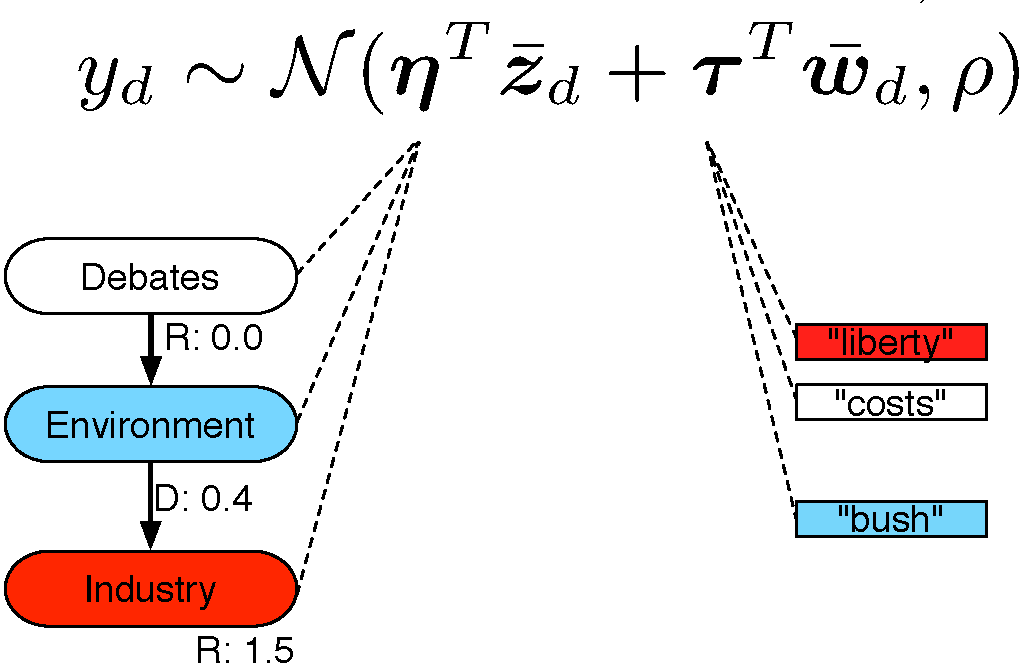
\includegraphics[width=.675\linewidth]{shlda/equation_2}}
    \only<4>{ 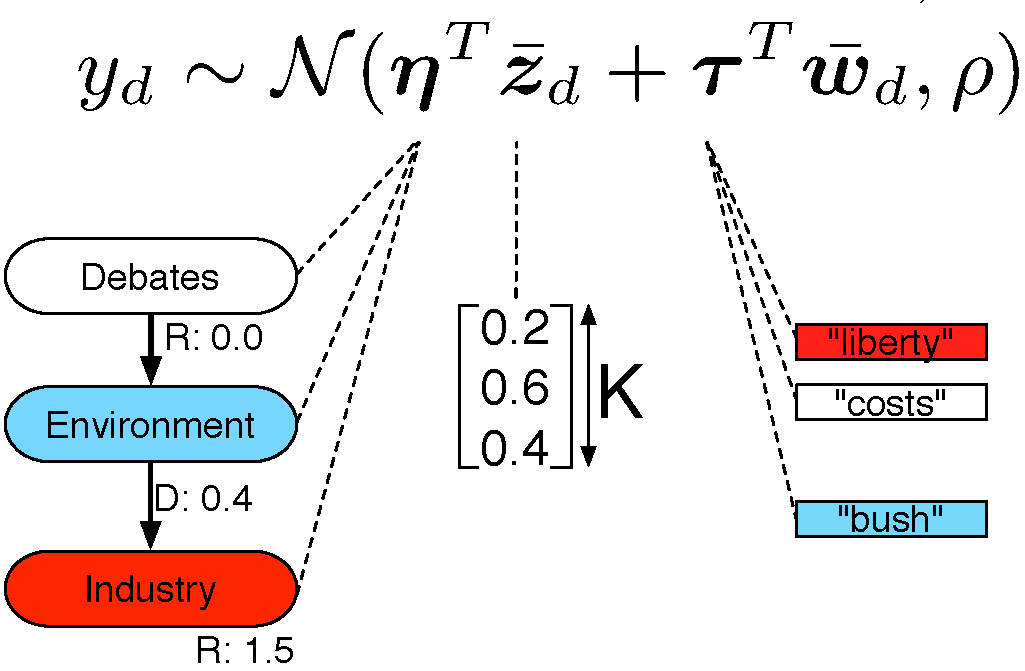
\includegraphics[width=.675\linewidth]{shlda/equation_3}}
    \only<5>{ 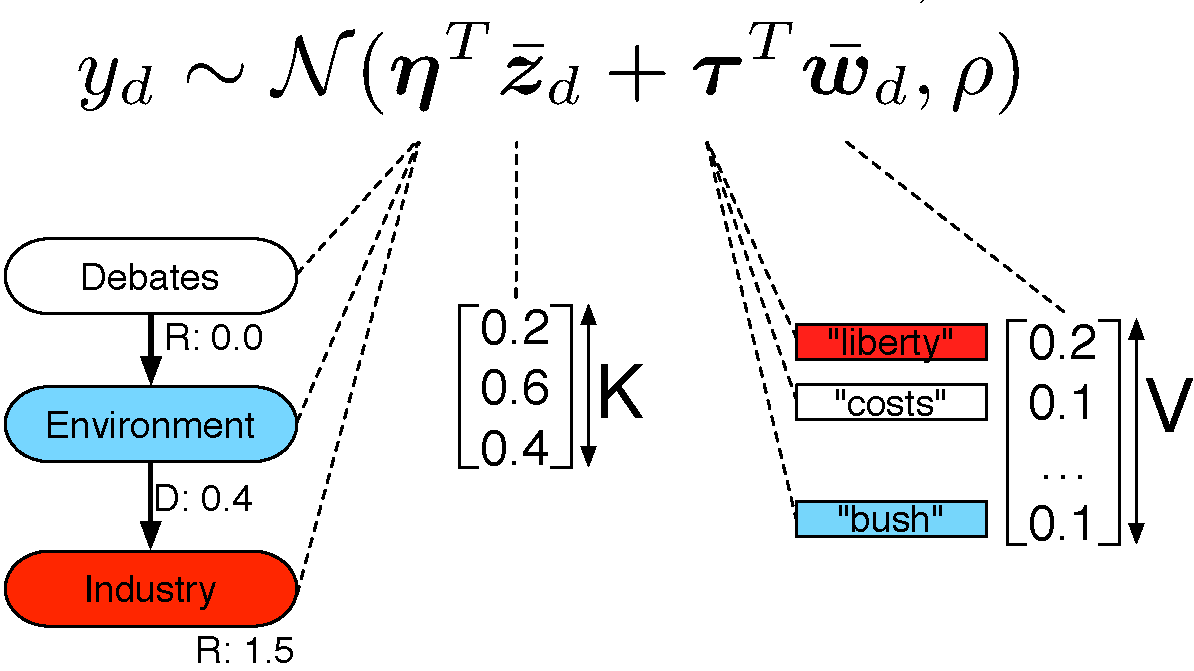
\includegraphics[width=.7\linewidth]{shlda/equation_4}}

 \begin{itemize}
    \item Some words have {\bf context-specific} contributions (topics)
    \item Some words have {\bf constant} contributions (words)
    \item Long noted for sentiment analysis
      \begin{itemize}
        \item ``Wonderful'': always good
          \item ``Unpredictable'': good for books, bad for steering
        \end{itemize}
    \end{itemize}


\end{frame}



\begin{frame}{Qualitative Results}
   \begin{center}
   \only<1>{ 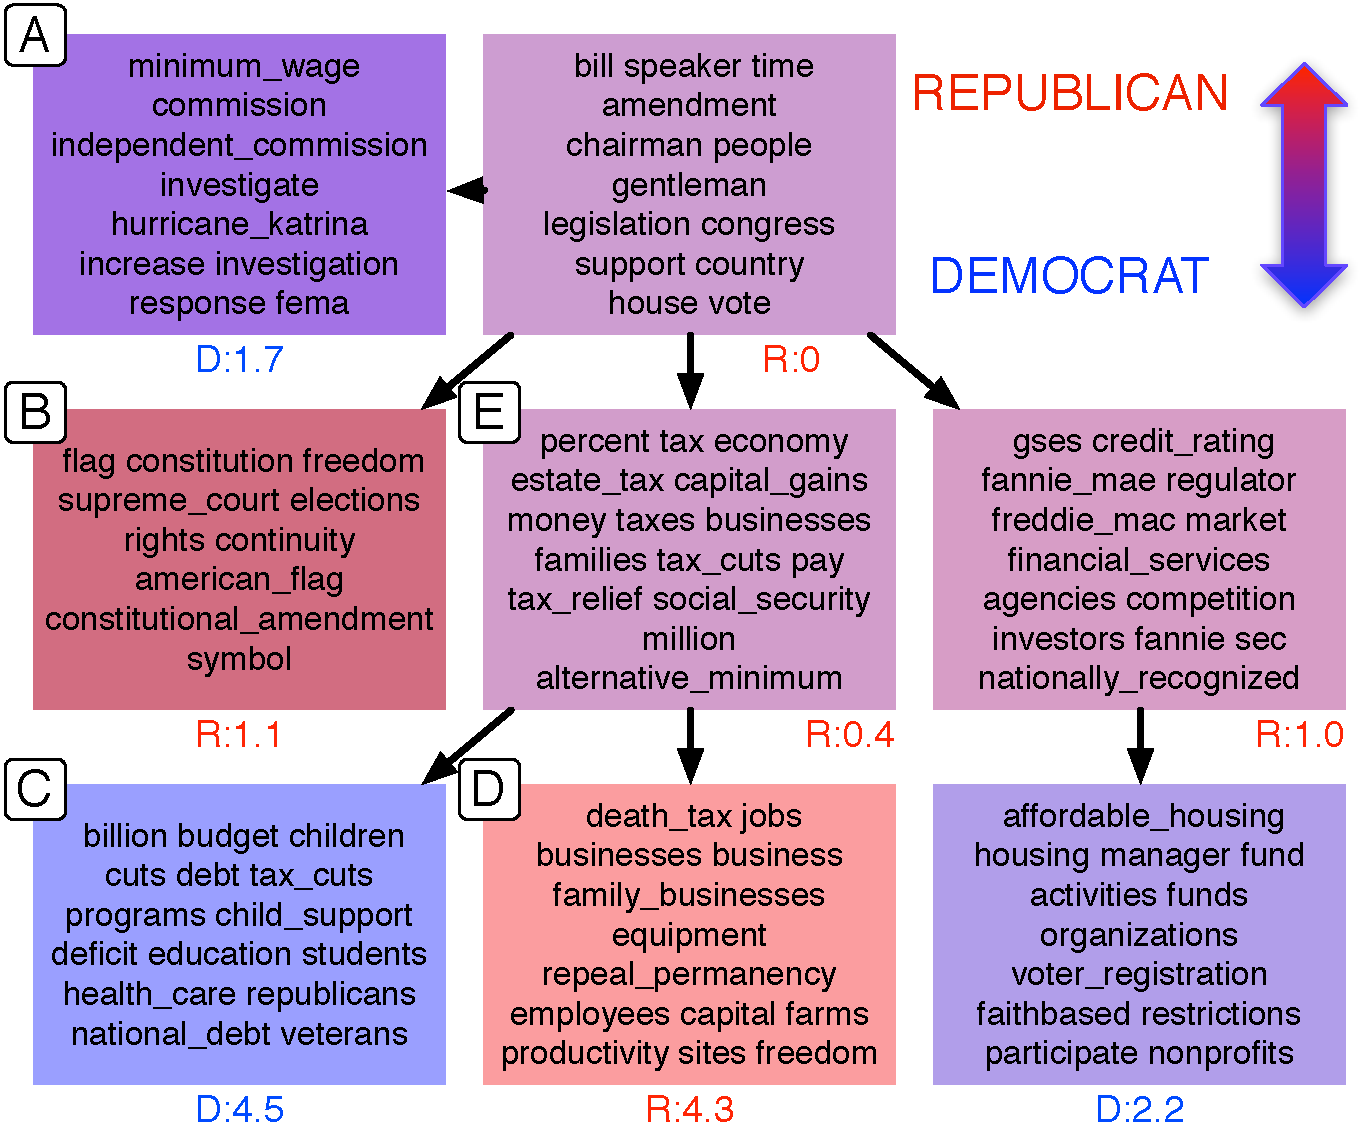
\includegraphics[width=0.8\linewidth]{shlda/ideology_topics}}
   \only<2>{ 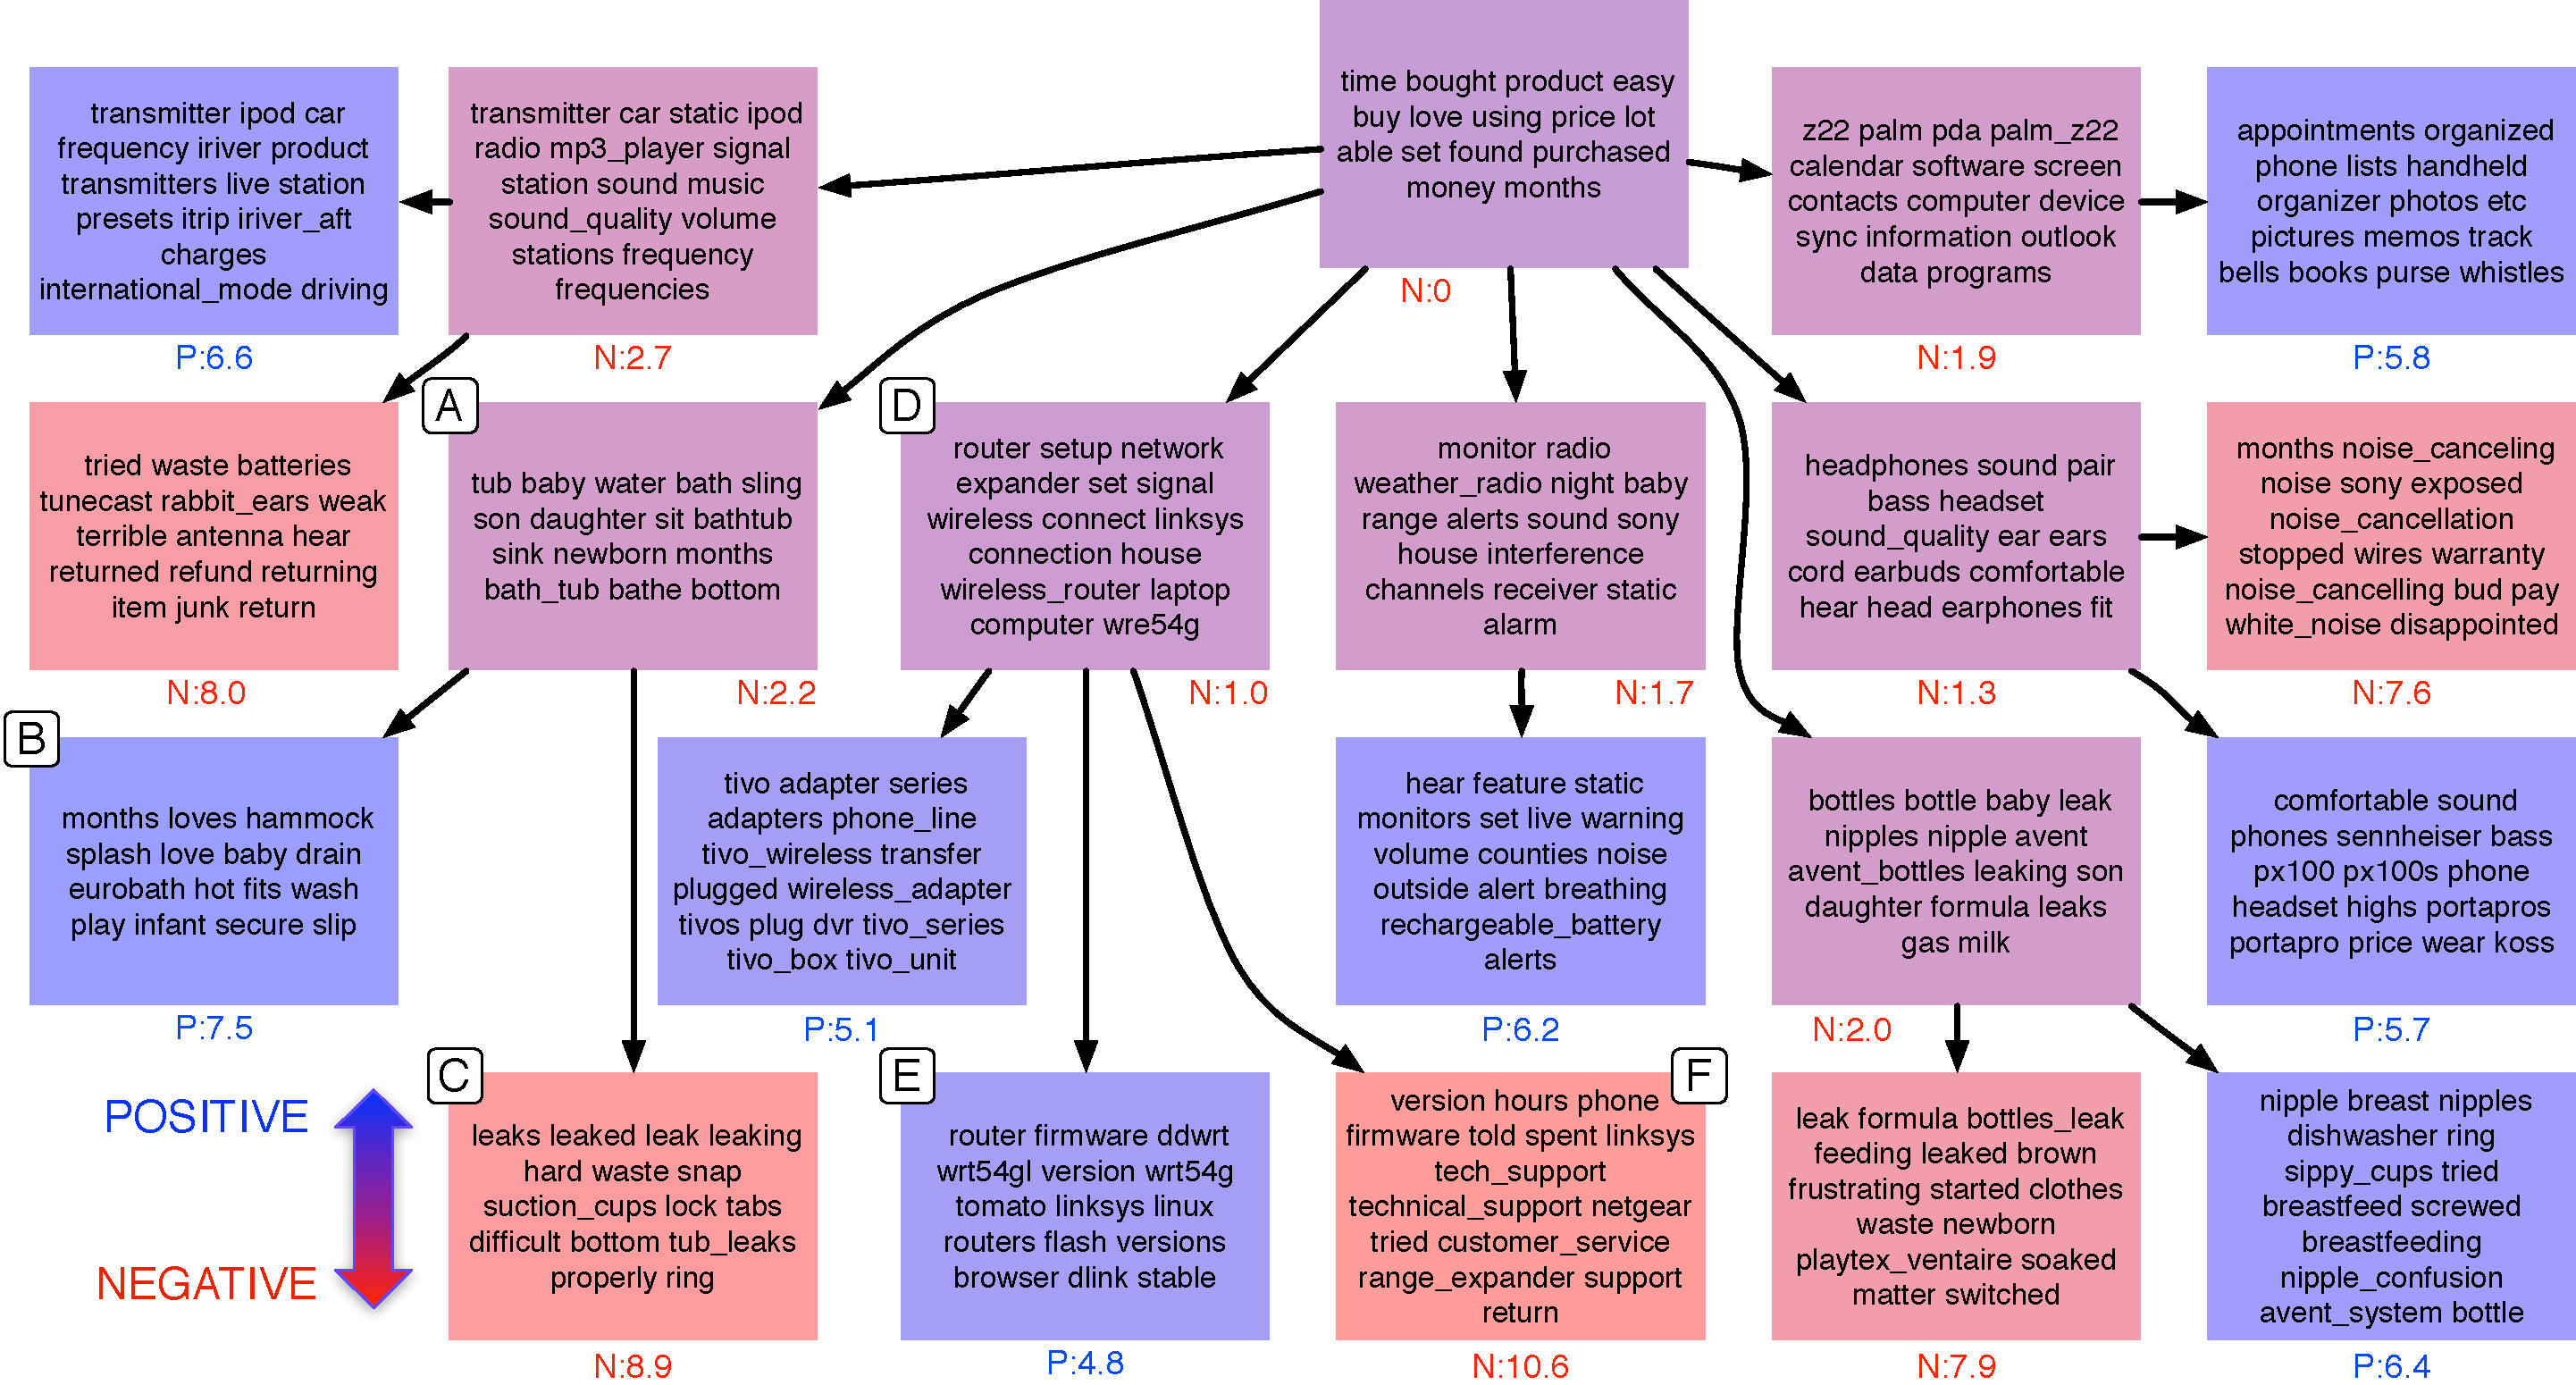
\includegraphics[width=1.0\linewidth]{shlda/amazon_topics}}
   \only<3>{ 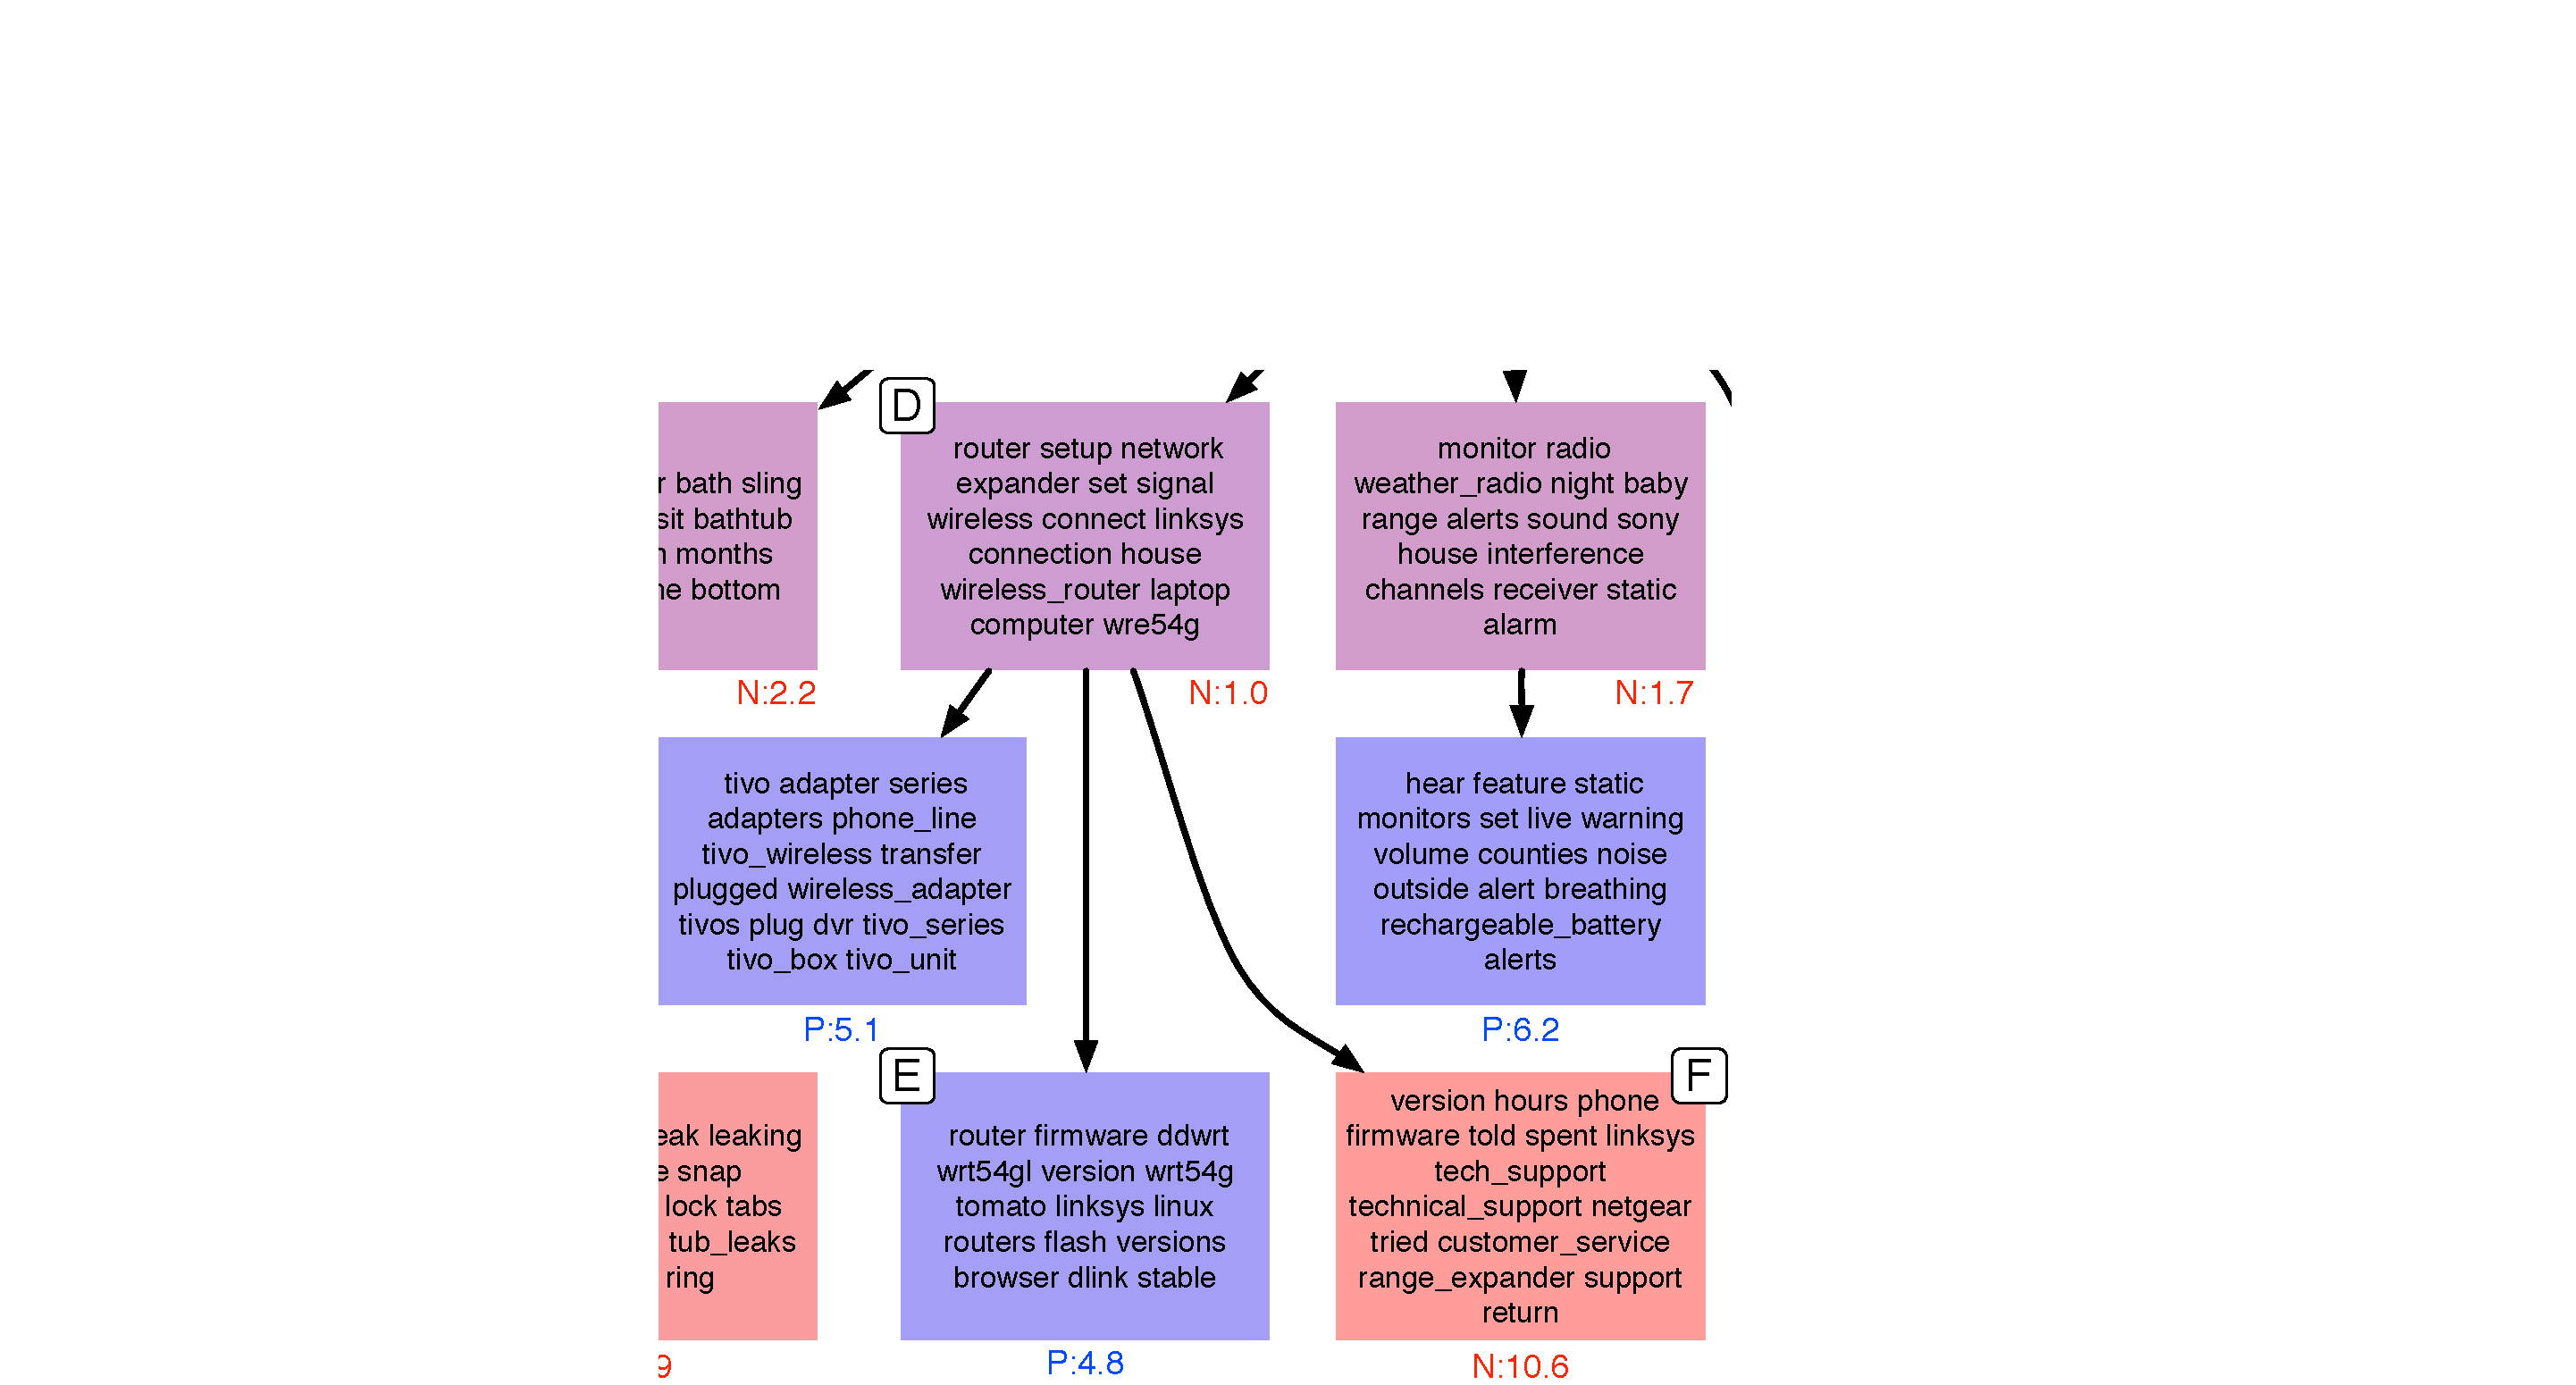
\includegraphics[width=0.7\linewidth]{shlda/amazon_topics_zoom}}
   \end{center}
\end{frame}

\begin{frame}{Quantitative Results}

\centering

\begin{tabular}{|c||c|c|c|c|}
  \hline
Models & Floor Debates & Amazon & Movie \\
  \hline
  $\textsc{svr-}\lda{}_{10}$     & $1.247$       & $1.241$ & $0.970$ \\
  $\textsc{svr-}\lda{}_{30}$     & $1.183$       & $1.091$ & $0.938$ \\
  $\textsc{svr-}\lda{}_{50}$     & $1.135$       & $1.130$ & $0.906$ \\
  {\textsc{svr-voc}}             & $1.467$       & $0.972$ & $0.681$\\
  {\textsc{svr-lda-voc}}         & $1.101$       & $0.965$ & $0.678$\\ \hline \hline
  $\textsc{mlr-}\lda{}_{10}$     & $1.151$       & $1.034$ & $0.957$ \\
  $\textsc{mlr-}\lda{}_{30}$     & $1.125$       & $1.065$ &$0.936$ \\
  $\textsc{mlr-}\lda{}_{50}$     & $1.081$       & $1.114$ & $0.914$ \\
  {\textsc{mlr-voc}}             & $1.124$       & $0.869$ & $0.721$\\
  {\textsc{mlr-lda-voc}}         & $1.120$       & $\bm {0.860}$ & $0.702$\\\hline \hline
  $\slda{}_{10}$                 & $1.145$       & $1.113$ & $0.953$\\
  $\slda{}_{30}$                 & $1.188$       & $1.146$ & $0.852$\\
  $\slda{}_{50}$                 & $1.184$       & $1.939$ & $0.772$\\ \hline \hline
  {\shlda{}}                     & $\bm {1.076}$ & $0.871$ & $\bm {0.673}$\\ \hline
\end{tabular}

Mean squared error averaged over 5 folds.
\end{frame}


\frame{

\begin{columns}

\column{.5\linewidth}

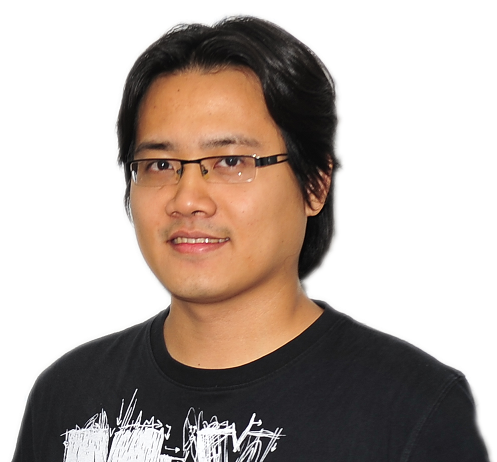
\includegraphics[width=.8\linewidth]{general_figures/an}

\column{.5\linewidth}

\begin{block}{ Tea Party in the House: A Hierarchical Ideal Point
    Topic Model and Its Application to Republican Legislators in the
    112th Congress}
Viet-An Nguyen, Jordan Boyd-Graber, Philip Resnik, and Kristina Miler.
Association for Computational Linguistics, 2015.
\end{block}

\end{columns}

}

\begin{frame}{Representing Elected Officials: Ideal Points}
  \gfxtp{dw_nominate}{.7}

  An essential tool in political science: distinguish trends and characterize subgroups
\end{frame}


\begin{frame}{Not everyone has a voting record}

  \begin{columns}
      \column{.25\linewidth}
        \gfxtp{carson}{.75}
        \gfxtp{fiorina}{.75}
      \column{.25\linewidth}
        \gfxtp{walker}{.75}
        \gfxtp{schwarzenegger}{.75}

    \column{.5\linewidth}
    \begin{itemize}
      \item Political scientists use voting records to predict alliances
      \item Not all candidates have a voting record
        \begin{itemize}
          \item Governors
          \item Entertainers
          \item CEOs
        \end{itemize}
        \pause
       \item But all politicians---by definition---talk
      \end{itemize}
  \end{columns}

\end{frame}


\frame{
    \frametitle{Hierarchical Ideal Point Topic Model: Intuition}
    \centering
    What are your thoughts on the issue of {\bf immigration}?
    \begin{figure}
    \centering
      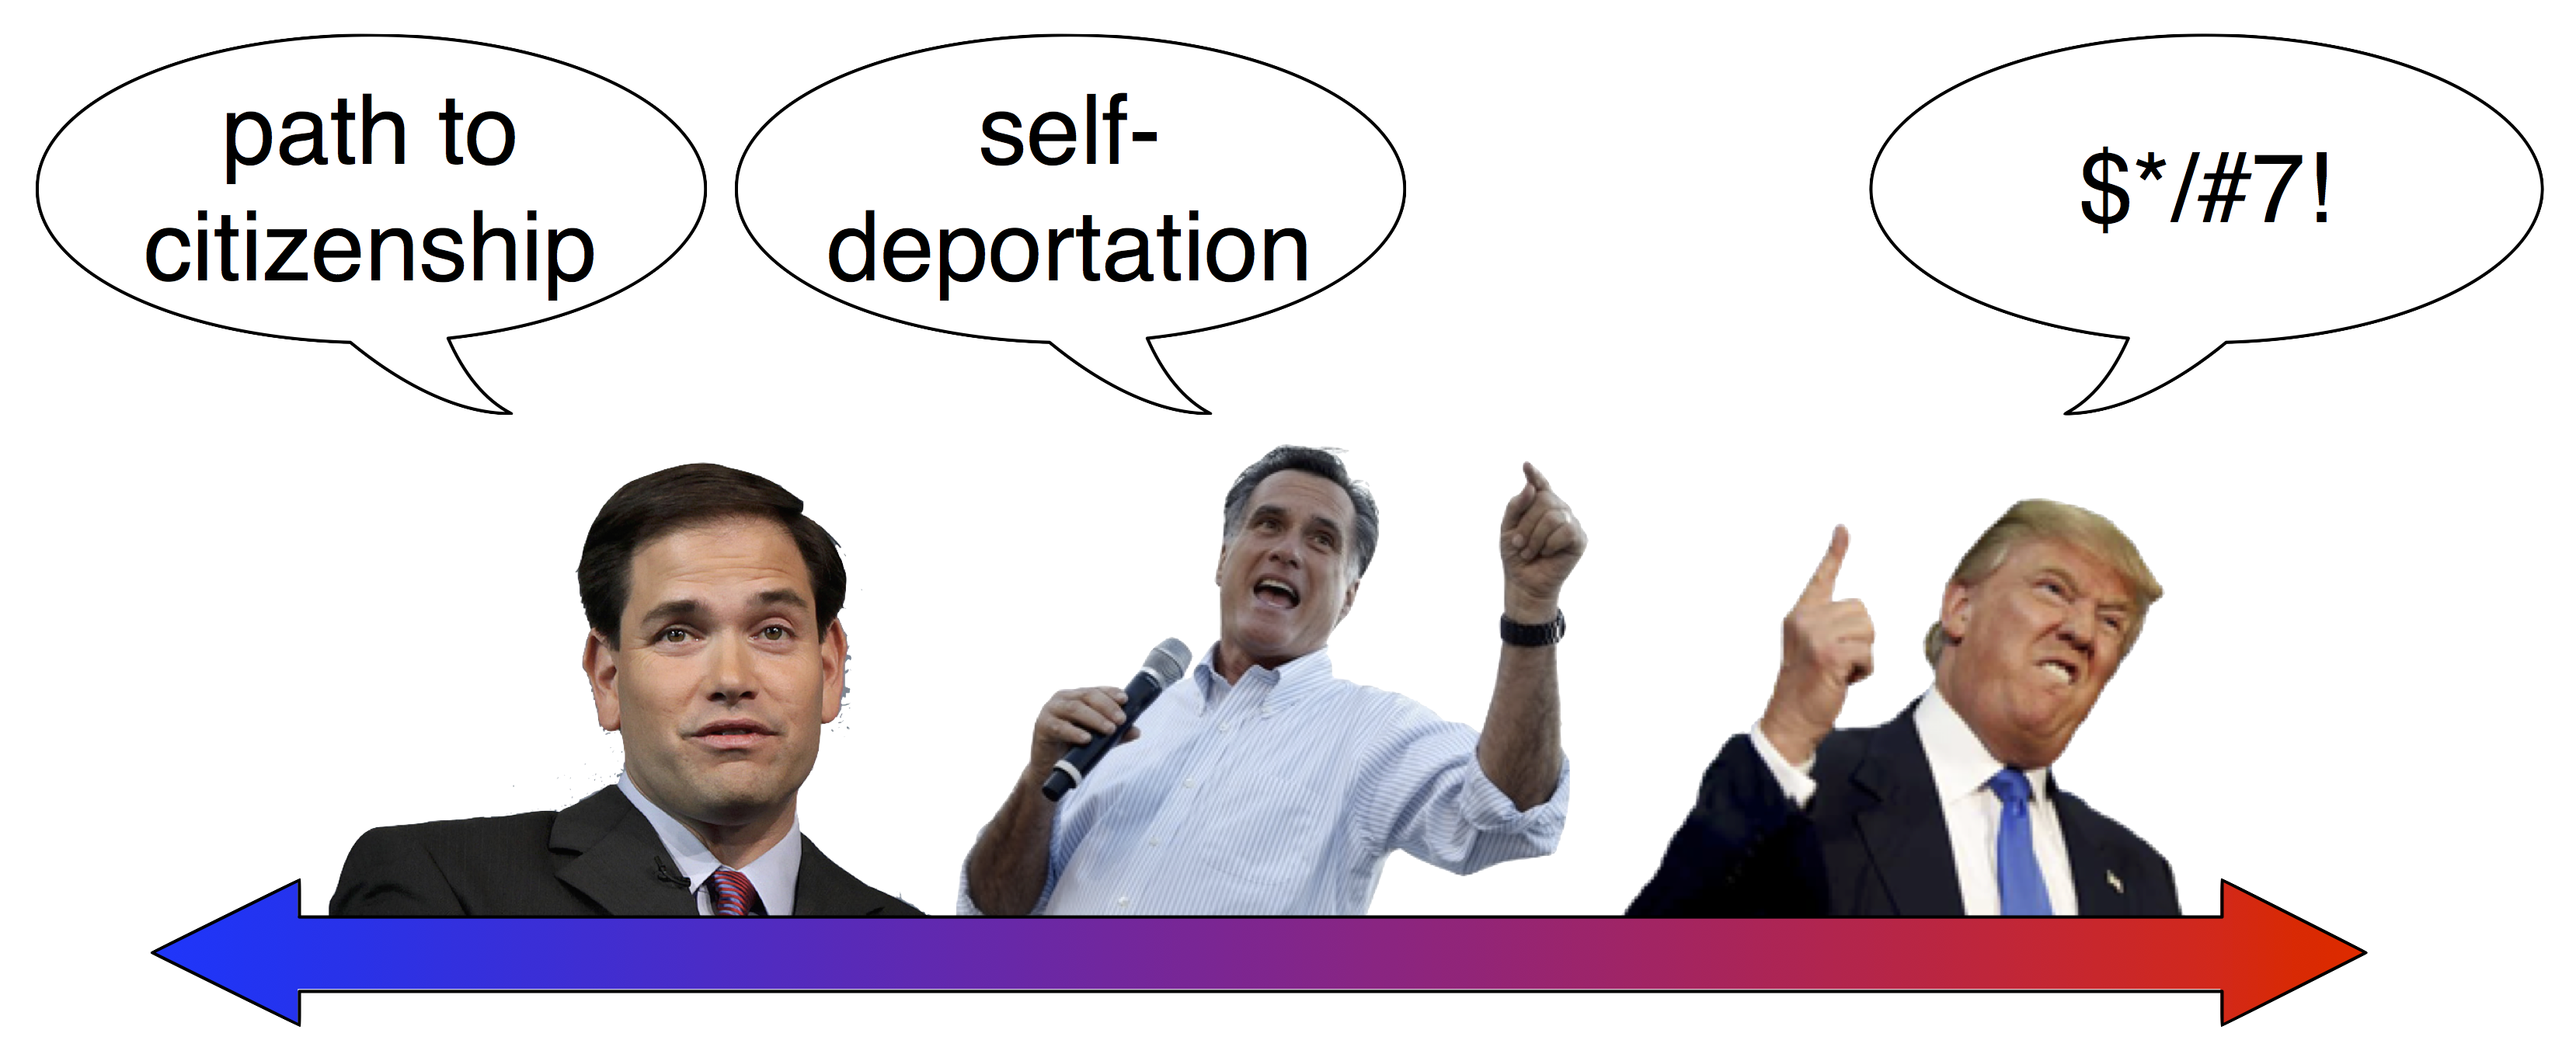
\includegraphics[width=\textwidth]{teaparty/figures/framing}
    \end{figure}
}

\frame{
    \frametitle{Hierarchical Ideal Point Topic Model}
      \centering
      \only<1>{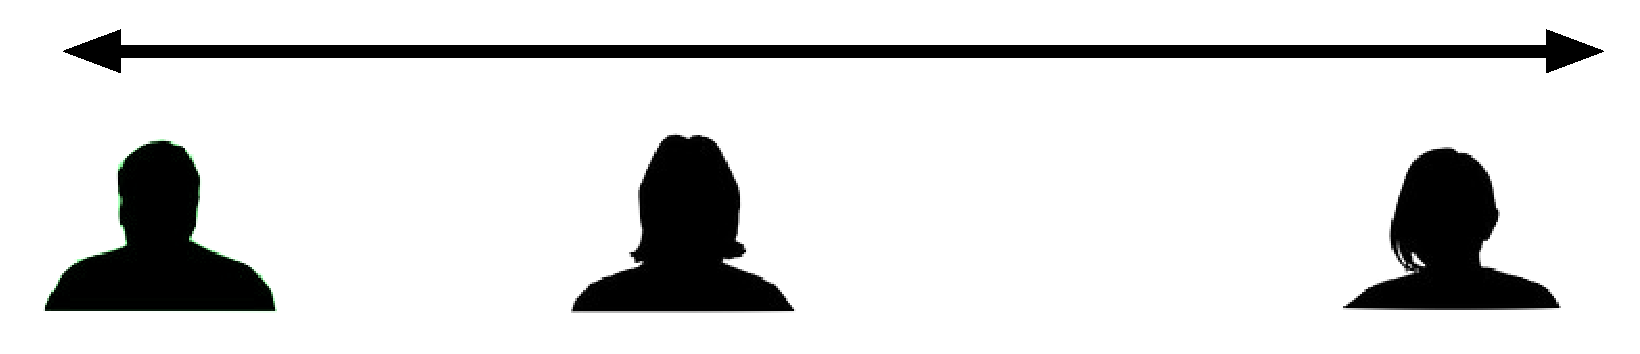
\includegraphics[width=.9\textwidth]{teaparty/figures/healthcare_intuition_1}}%
      \only<2>{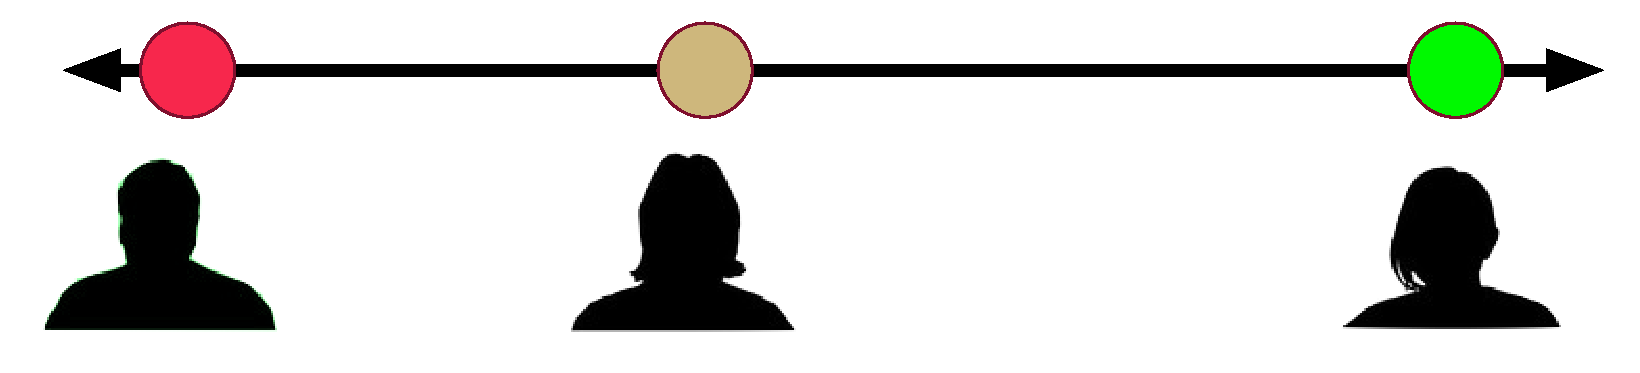
\includegraphics[width=.9\textwidth]{teaparty/figures/healthcare_intuition_2}}%
      \only<3>{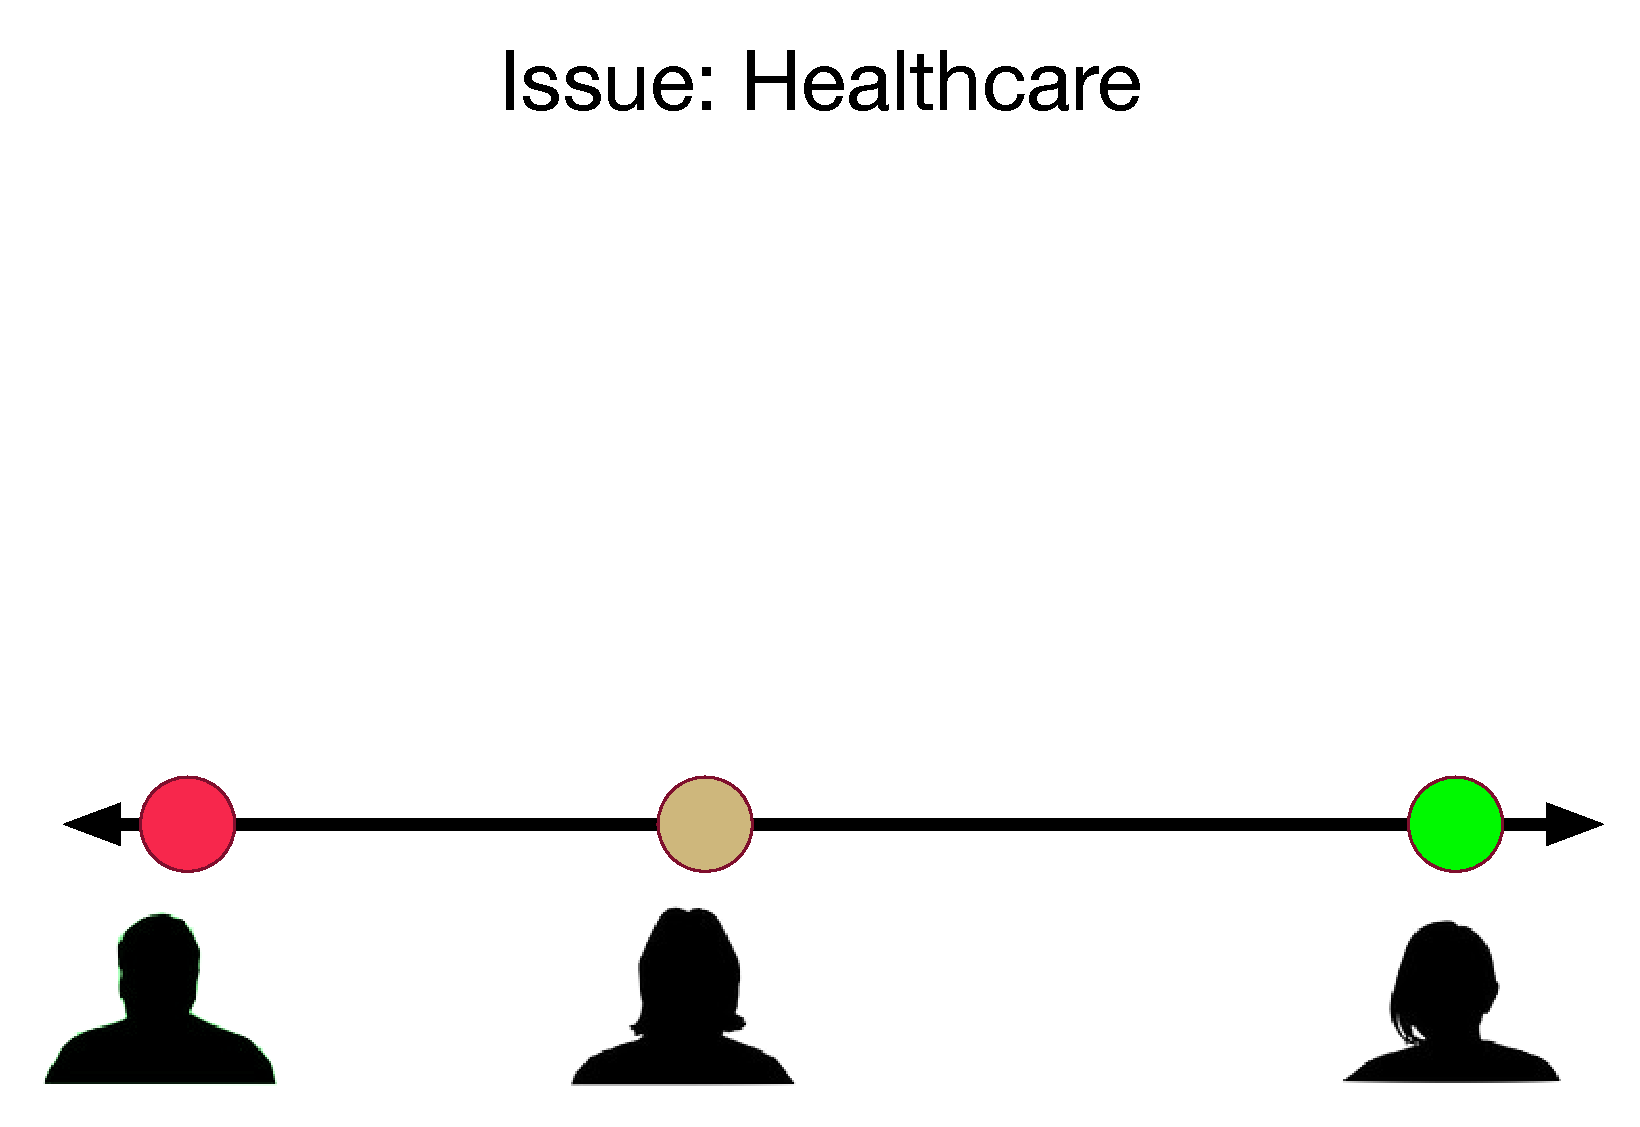
\includegraphics[width=.9\textwidth]{teaparty/figures/healthcare_intuition_3}}%
      \only<4>{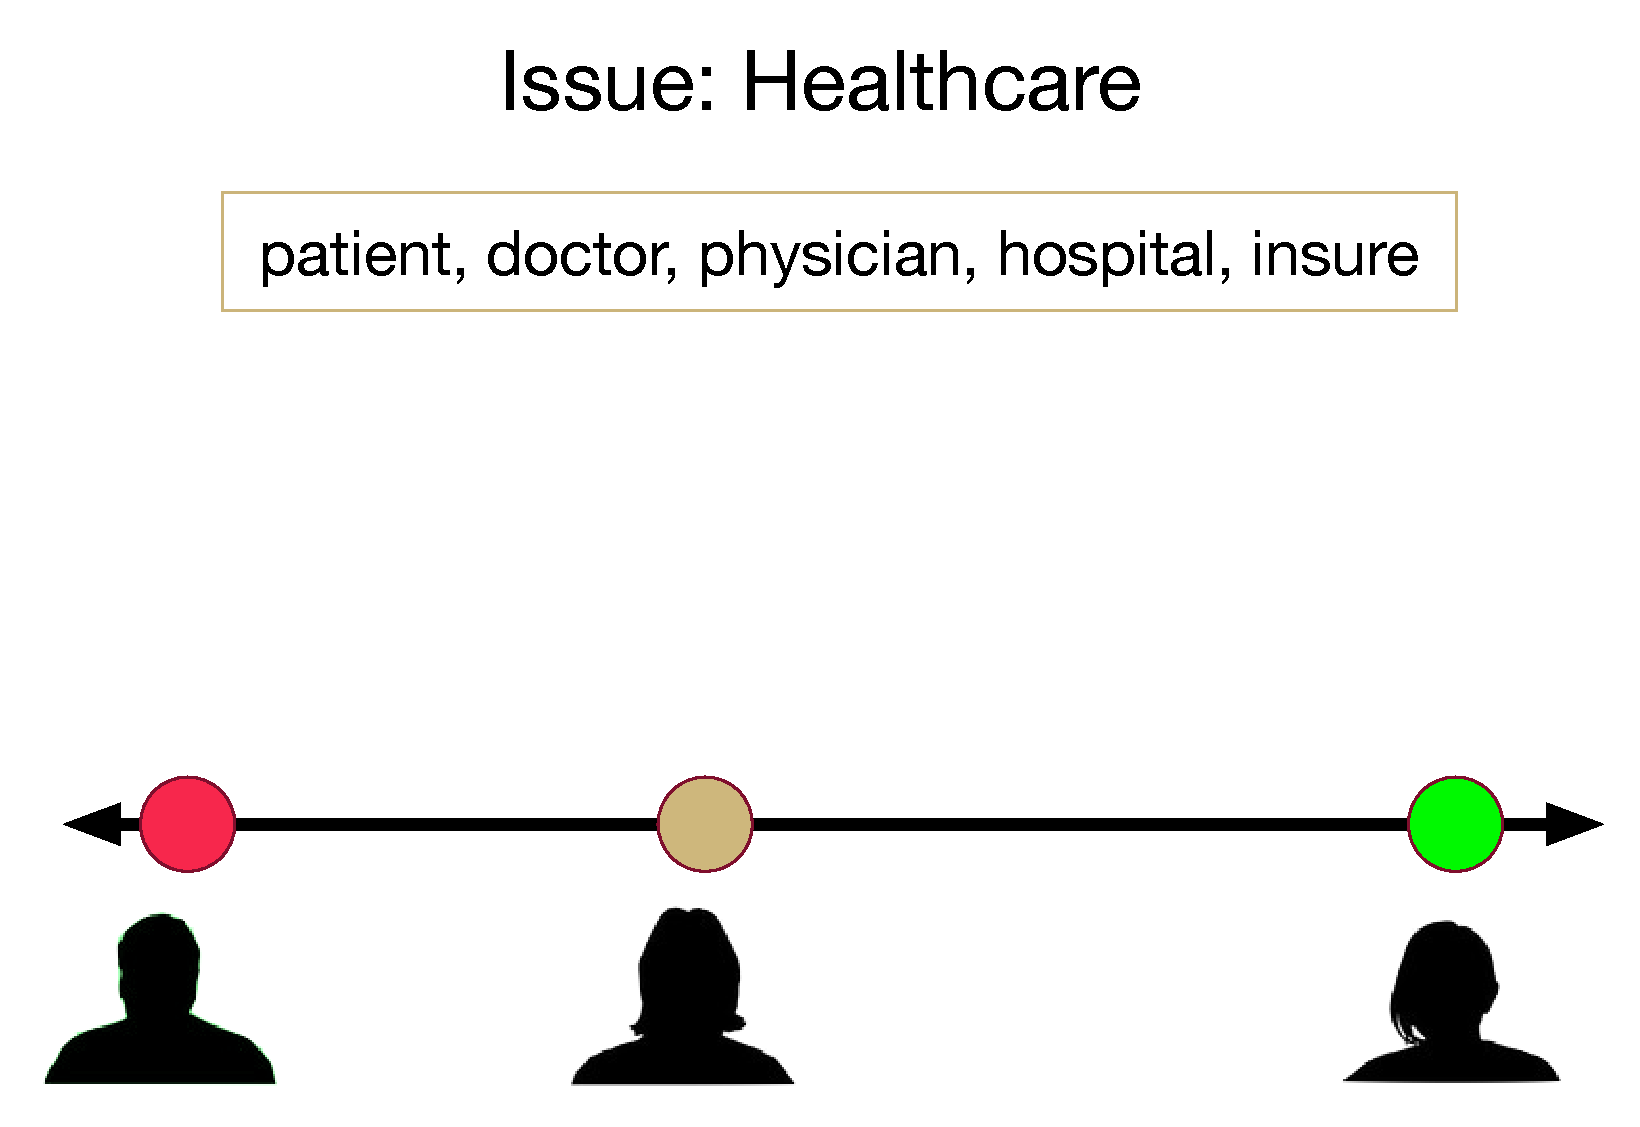
\includegraphics[width=.9\textwidth]{teaparty/figures/healthcare_intuition_4}}%
      \only<5>{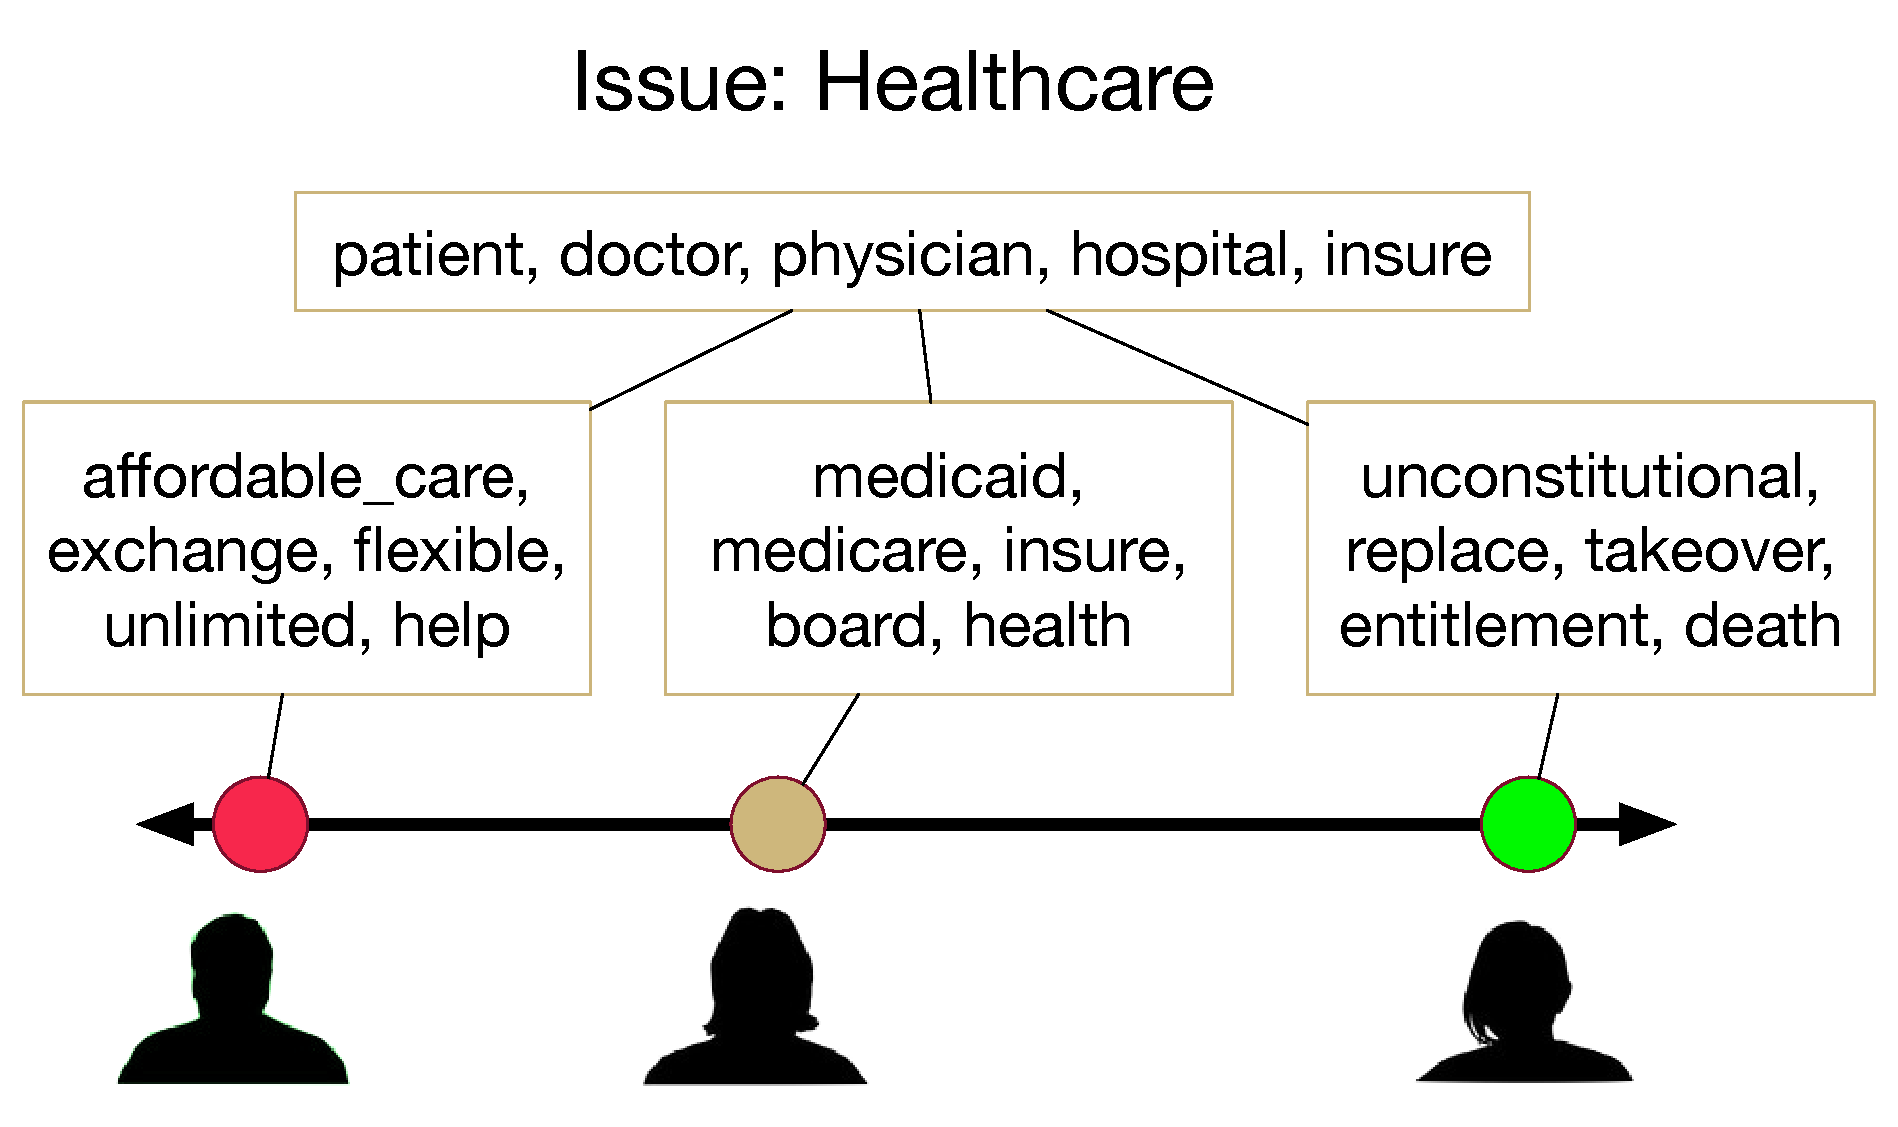
\includegraphics[width=.9\textwidth]{teaparty/figures/healthcare_intuition_5}}%
}

\frame{
    \frametitle{Tea Party Caucus Membership Prediction}
    \begin{block}{Experiment setup}
    \begin{itemize}
    \small
      \item Task: Binary classification of whether a legislator is a member of the Tea Party Caucus
      \item Evaluation metric: AUC-ROC
      \item Classifier: SVM$^{light}$
      \item Five-fold stratified cross-validation
    \end{itemize}
    \end{block}

    \pause

    \begin{block}{Features}
    \begin{itemize}
    \small
      \item Text-based features: normalized term frequency (\textbf{TF}) and \textbf{TF-IDF}
      \item \textbf{Vote}: binary features
      \item \textbf{HIPTM}: features extracted from our model including
      \begin{itemize}
        \item $K$-dim ideal point $u \subtwo ak$ estimated from both votes and text
        \item $K$-dim ideal point estimated from text only $\bm \eta_k^T \hat{\bm \psi} \subtwo ak$
        \item $B$ probabilities estimating $a$'s votes $\Phi(x_b \sum_{k=1}^K \vartheta \subtwo bk u \subtwo ak +
          y_b)$
      \end{itemize}
    \end{itemize}
    \end{block}
}

\frame{
    \frametitle{Tea Party Caucus Membership Prediction: Votes \& Text}
    \begin{center}
        \includegraphics<1>[width=\textwidth]{teaparty/figures/s5/votetext_1}
        \includegraphics<2>[width=\textwidth]{teaparty/figures/s5/votetext_2}
        \includegraphics<3>[width=\textwidth]{teaparty/figures/s5/votetext_3}
        \includegraphics<4>[width=\textwidth]{teaparty/figures/s5/votetext_4}
        \includegraphics<5>[width=\textwidth]{teaparty/figures/s5/votetext_5}
        \includegraphics<6>[width=\textwidth]{teaparty/figures/s5/votetext_6}
    \end{center}
}

\frame{
    \frametitle{Tea Party Caucus Membership Prediction: Text Only}
      \begin{center}
        \includegraphics<1>[width=\textwidth]{teaparty/figures/s5/textonly_1}
        \includegraphics<2->[width=\textwidth]{teaparty/figures/s5/textonly_2}
      \end{center}

%      \begin{block}{}
%        Vote-based features are not needed at test time, so this model makes it possible to do better
%prediction even for people who have no voting record in Congress
%        \begin{itemize}
%          \item e.g., new members of Congress or political candidates.
%        \end{itemize}
%      \end{block}
}


\begin{frame}{Predicting Conflict}
	\only<1>{\gfxtp{polarization_1}{.7}}
	\only<2>{\gfxtp{polarization_2}{.7}}
	\only<3>{\gfxtp{polarization_3}{.7}}
	\only<4>{\gfxtp{polarization_4}{.7}}
\end{frame}

\begin{frame}{}

  \begin{columns}
    \column{.5\linewidth}
        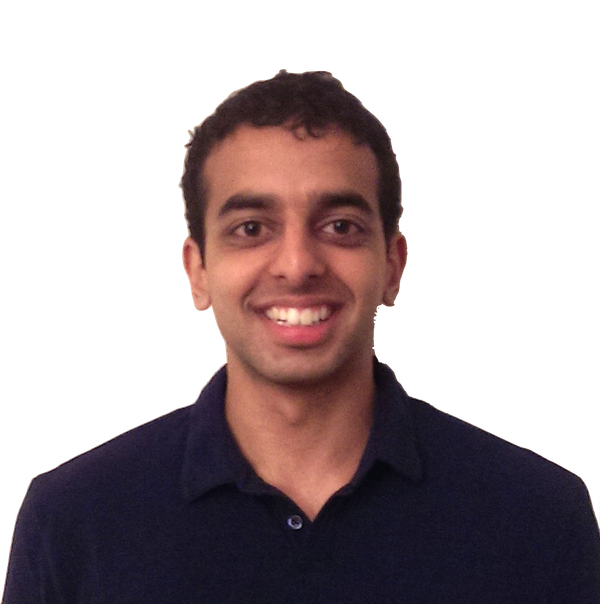
\includegraphics[width=0.7\linewidth]{general_figures/mohit}
    \column{.5\linewidth}
        \begin{block}{ {\bf \href{http://cs.colorado.edu/~jbg//docs/2014_emnlp_qb_rnn.pdf}{Feuding Families and Former Friends: Unsupervised Learning for Dynamic Fictional Relationships}}}
\underline{\href{http://cs.umd.edu/~miyyer/}{Mohit Iyyer}},Anupam Guha, Snigdha Chaturvedi, {\bf Jordan Boyd-Graber}, and Hal {Daum\'{e} III}.  \emph{NAACL}, 2014
        \end{block}
Best Paper Award
  \end{columns}
\end{frame}



\begin{frame}[plain]
\vspace*{-1pt}
\only<1>{\makebox[\linewidth]{\includegraphics[page=1,width=\paperwidth]{relationships/motivation_and_ex}}}
\only<2>{\makebox[\linewidth]{\includegraphics[page=2,width=\paperwidth]{relationships/motivation_and_ex}}}
\only<3>{\makebox[\linewidth]{\includegraphics[page=3,width=\paperwidth]{relationships/motivation_and_ex}}}
\only<4>{\makebox[\linewidth]{\includegraphics[page=4,width=\paperwidth]{relationships/motivation_and_ex}}}
\only<5>{\makebox[\linewidth]{\includegraphics[page=5,width=\paperwidth]{relationships/motivation_and_ex}}}
\only<6>{\makebox[\linewidth]{\includegraphics[page=6,width=\paperwidth]{relationships/motivation_and_ex}}}
\only<7>{\makebox[\linewidth]{\includegraphics[page=7,width=\paperwidth]{relationships/motivation_and_ex}}}
\only<8>{\makebox[\linewidth]{\includegraphics[page=8,width=\paperwidth]{relationships/motivation_and_ex}}}
\only<9>{\makebox[\linewidth]{\includegraphics[page=9,width=\paperwidth]{relationships/motivation_and_ex}}}
\only<10>{\makebox[\linewidth]{\includegraphics[page=10,width=\paperwidth]{relationships/motivation_and_ex}}}
\only<11>{\makebox[\linewidth]{\includegraphics[page=11,width=\paperwidth]{relationships/motivation_and_ex}}}
\only<12>{\makebox[\linewidth]{\includegraphics[page=12,width=\paperwidth]{relationships/motivation_and_ex}}}
\only<13>{\makebox[\linewidth]{\includegraphics[page=13,width=\paperwidth]{relationships/motivation_and_ex}}}
\only<14>{\makebox[\linewidth]{\includegraphics[page=14,width=\paperwidth]{relationships/motivation_and_ex}}}
\only<15>{\makebox[\linewidth]{\includegraphics[page=15,width=\paperwidth]{relationships/motivation_and_ex}}}
\only<16>{\makebox[\linewidth]{\includegraphics[page=16,width=\paperwidth]{relationships/motivation_and_ex}}}
\only<17>{\makebox[\linewidth]{\includegraphics[page=17,width=\paperwidth]{relationships/motivation_and_ex}}}
\only<18>{\makebox[\linewidth]{\includegraphics[page=18,width=\paperwidth]{relationships/motivation_and_ex}}}
\only<19>{\makebox[\linewidth]{\includegraphics[page=19,width=\paperwidth]{relationships/motivation_and_ex}}}
\only<20>{\makebox[\linewidth]{\includegraphics[page=20,width=\paperwidth]{relationships/motivation_and_ex}}}
\only<21>{\makebox[\linewidth]{\includegraphics[page=21,width=\paperwidth]{relationships/motivation_and_ex}}}
\end{frame}

\begin{frame}[plain]
\vspace*{-1pt}
\only<1>{\makebox[\linewidth]{\includegraphics[page=1,width=\paperwidth]{relationships/dataset}}}
\only<2>{\makebox[\linewidth]{\includegraphics[page=2,width=\paperwidth]{relationships/dataset}}}
\only<3>{\makebox[\linewidth]{\includegraphics[page=3,width=\paperwidth]{relationships/dataset}}}
\only<4>{\makebox[\linewidth]{\includegraphics[page=4,width=\paperwidth]{relationships/dataset}}}
\only<5>{\makebox[\linewidth]{\includegraphics[page=5,width=\paperwidth]{relationships/dataset}}}
\end{frame}

\begin{frame}[plain]
\vspace*{-1pt}
\only<1>{\makebox[\linewidth]{\includegraphics[page=1,width=\paperwidth]{relationships/model}}}
\only<2>{\makebox[\linewidth]{\includegraphics[page=2,width=\paperwidth]{relationships/model}}}
\only<3>{\makebox[\linewidth]{\includegraphics[page=3,width=\paperwidth]{relationships/model}}}
\only<4>{\makebox[\linewidth]{\includegraphics[page=4,width=\paperwidth]{relationships/model}}}
\only<5>{\makebox[\linewidth]{\includegraphics[page=5,width=\paperwidth]{relationships/model}}}
\only<6>{\makebox[\linewidth]{\includegraphics[page=6,width=\paperwidth]{relationships/model}}}
\only<7>{\makebox[\linewidth]{\includegraphics[page=7,width=\paperwidth]{relationships/model}}}
\only<8>{\makebox[\linewidth]{\includegraphics[page=8,width=\paperwidth]{relationships/model}}}
\only<9>{\makebox[\linewidth]{\includegraphics[page=9,width=\paperwidth]{relationships/model}}}
\only<10>{\makebox[\linewidth]{\includegraphics[page=10,width=\paperwidth]{relationships/model}}}
\only<11>{\makebox[\linewidth]{\includegraphics[page=11,width=\paperwidth]{relationships/model}}}
\only<12>{\makebox[\linewidth]{\includegraphics[page=12,width=\paperwidth]{relationships/model}}}
\end{frame}

\begin{frame}{Doesn't this look like topic models?}

  \begin{itemize}
    \item Descriptors resemble topics
    \item Topic models capture similar phenomena
      \begin{itemize}
        \item Hidden Topic Markov Model (Gruber et al., 2007)
        \item Nubbi (Chang et al., 2009)
      \end{itemize}
    \item Topic models touted for their interpretability
    \item Let's compare apples to apples
  \end{itemize}

\end{frame}

\begin{frame}[plain]
\vspace*{-1pt}
\only<1>{\makebox[\linewidth]{\includegraphics[page=1,width=\paperwidth]{relationships/coherence}}}
\only<2>{\makebox[\linewidth]{\includegraphics[page=2,width=\paperwidth]{relationships/coherence}}}
\only<3>{\makebox[\linewidth]{\includegraphics[page=3,width=\paperwidth]{relationships/coherence}}}
\only<4>{\makebox[\linewidth]{\includegraphics[page=4,width=\paperwidth]{relationships/coherence}}}
\only<5>{\makebox[\linewidth]{\includegraphics[page=5,width=\paperwidth]{relationships/coherence}}}
\only<6>{\makebox[\linewidth]{\includegraphics[page=6,width=\paperwidth]{relationships/coherence}}}
\only<7>{\makebox[\linewidth]{\includegraphics[page=7,width=\paperwidth]{relationships/coherence}}}
\end{frame}


\begin{frame}[plain]
\vspace*{-1pt}
\only<1>{\makebox[\linewidth]{\includegraphics[page=1,width=\paperwidth]{relationships/trajectories}}}
\only<2>{\makebox[\linewidth]{\includegraphics[page=2,width=\paperwidth]{relationships/trajectories}}}
\only<3>{\makebox[\linewidth]{\includegraphics[page=3,width=\paperwidth]{relationships/trajectories}}}
\only<4>{\makebox[\linewidth]{\includegraphics[page=4,width=\paperwidth]{relationships/trajectories}}}
\only<5>{\makebox[\linewidth]{\includegraphics[page=5,width=\paperwidth]{relationships/trajectories}}}
\only<6>{\makebox[\linewidth]{\includegraphics[page=6,width=\paperwidth]{relationships/trajectories}}}
\only<7>{\makebox[\linewidth]{\includegraphics[page=7,width=\paperwidth]{relationships/trajectories}}}
\end{frame}

\begin{frame}{Conclusion}


  \begin{itemize}
    \item New model for summarizing relationships
    \item Application: Matching plot summaries to book titles
    \item Methodology: Interpretability of deep learning dictionaries
  \end{itemize}

\end{frame}


% Update paper http://www.umiacs.umd.edu/~jbg/docs/
\begin{frame}{}

  \begin{columns}
    \column{.5\linewidth}
        \includegraphics[width=0.7\linewidth]{general_figures/vlad}
    \column{.5\linewidth}
        \begin{block}{{\bf
              \href{http://cs.colorado.edu/~jbg//docs/2015_acl_diplomacy.pdf}{Linguistic Harbingers of Betrayal: A Case Study on an Online Strategy Game}}}

          Vlad Niculae, Srijan Kumar, Jordan Boyd-Graber, and Cristian
          Danescu-Niculescu-Mizil. \emph{Association for Computational Linguistics}, 2015
        \end{block}

  \end{columns}
\end{frame}


\begin{frame}[plain]
\vspace*{-1pt}
\only<1>{\makebox[\linewidth]{\includegraphics[page=1,width=\paperwidth]{diplomacy/betrayal-slides}}}
\only<2>{\makebox[\linewidth]{\includegraphics[page=2,width=\paperwidth]{diplomacy/betrayal-slides}}}
\only<3>{\makebox[\linewidth]{\includegraphics[page=3,width=\paperwidth]{diplomacy/betrayal-slides}}}
\only<4>{\makebox[\linewidth]{\includegraphics[page=4,width=\paperwidth]{diplomacy/betrayal-slides}}}
\only<5>{\makebox[\linewidth]{\includegraphics[page=5,width=\paperwidth]{diplomacy/betrayal-slides}}}
\only<6>{\makebox[\linewidth]{\includegraphics[page=6,width=\paperwidth]{diplomacy/betrayal-slides}}}
\only<7>{\makebox[\linewidth]{\includegraphics[page=7,width=\paperwidth]{diplomacy/betrayal-slides}}}
\only<8>{\makebox[\linewidth]{\includegraphics[page=8,width=\paperwidth]{diplomacy/betrayal-slides}}}
\only<9>{\makebox[\linewidth]{\includegraphics[page=9,width=\paperwidth]{diplomacy/betrayal-slides}}}
\only<10>{\makebox[\linewidth]{\includegraphics[page=10,width=\paperwidth]{diplomacy/betrayal-slides}}}
\only<11>{\makebox[\linewidth]{\includegraphics[page=11,width=\paperwidth]{diplomacy/betrayal-slides}}}
\only<12>{\makebox[\linewidth]{\includegraphics[page=12,width=\paperwidth]{diplomacy/betrayal-slides}}}
\only<13>{\makebox[\linewidth]{\includegraphics[page=13,width=\paperwidth]{diplomacy/betrayal-slides}}}
\only<14>{\makebox[\linewidth]{\includegraphics[page=14,width=\paperwidth]{diplomacy/betrayal-slides}}}
\only<15>{\makebox[\linewidth]{\includegraphics[page=15,width=\paperwidth]{diplomacy/betrayal-slides}}}
\only<16>{\makebox[\linewidth]{\includegraphics[page=16,width=\paperwidth]{diplomacy/betrayal-slides}}}
\only<17>{\makebox[\linewidth]{\includegraphics[page=17,width=\paperwidth]{diplomacy/betrayal-slides}}}
\only<18>{\makebox[\linewidth]{\includegraphics[page=18,width=\paperwidth]{diplomacy/betrayal-slides}}}
\only<19>{\makebox[\linewidth]{\includegraphics[page=19,width=\paperwidth]{diplomacy/betrayal-slides}}}
\only<20>{\makebox[\linewidth]{\includegraphics[page=20,width=\paperwidth]{diplomacy/betrayal-slides}}}
\only<21>{\makebox[\linewidth]{\includegraphics[page=21,width=\paperwidth]{diplomacy/betrayal-slides}}}
\end{frame}

\begin{frame}[plain]
\vspace*{-1pt}
\only<1>{\makebox[\linewidth]{\includegraphics[page=1,width=\paperwidth]{diplomacy/betrayal-results}}}
\only<2>{\makebox[\linewidth]{\includegraphics[page=2,width=\paperwidth]{diplomacy/betrayal-results}}}
\only<3>{\makebox[\linewidth]{\includegraphics[page=3,width=\paperwidth]{diplomacy/betrayal-results}}}
\only<4>{\makebox[\linewidth]{\includegraphics[page=4,width=\paperwidth]{diplomacy/betrayal-results}}}
\only<5>{\makebox[\linewidth]{\includegraphics[page=5,width=\paperwidth]{diplomacy/betrayal-results}}}
\only<6>{\makebox[\linewidth]{\includegraphics[page=6,width=\paperwidth]{diplomacy/betrayal-results}}}
\only<7>{\makebox[\linewidth]{\includegraphics[page=7,width=\paperwidth]{diplomacy/betrayal-results}}}
\only<8>{\makebox[\linewidth]{\includegraphics[page=8,width=\paperwidth]{diplomacy/betrayal-results}}}
\only<9>{\makebox[\linewidth]{\includegraphics[page=9,width=\paperwidth]{diplomacy/betrayal-results}}}
\only<10>{\makebox[\linewidth]{\includegraphics[page=10,width=\paperwidth]{diplomacy/betrayal-results}}}
\only<11>{\makebox[\linewidth]{\includegraphics[page=11,width=\paperwidth]{diplomacy/betrayal-results}}}

\end{frame}


%\input{topicshift-an/topicshift-an}

        \begin{frame}{Framing, relationships, and betrayal}

           \begin{itemize}
              \item Rethinking {\bf evaluation}
                \item Revealing {\bf internal state}
                    \item Enabling {\bf interdisciplinary collaborations}
            \end{itemize}

\end{frame}



\frame{
  \frametitle{Ongoing and Future Work}

  \begin{itemize}
        \item Embedding interactivity in applications
    \item Visualizations to measure machine learning explainability
    \item Using morphology in infinite representations
    \item Multilingual analysis
    \end{itemize}
}

\frame{
  \frametitle{But wait, there's more!}

\begin{columns}

  \column{.5\linewidth}
    \begin{block}{Question Answering}
    \centering
        \includegraphics[width=0.5\linewidth]{qb/jennings_handshake} \\
     \small
       \cite{iyyer-15,He:Boyd-Graber:Daume-III-2016}
    \end{block}


    \begin{block}{Machine Translation}
      \begin{center}
        \includegraphics[width=0.5\linewidth]{simtrans/computer-interpreter} \\
      \cite{Hu:Zhai:Eidelman:Boyd-Graber-2014,II:He:Boyd-Graber:Morgan-2014}
       \end{center}
    \vspace{-.4cm}
    \end{block}

  \column{.5\linewidth}



    \begin{block}{Assistive Technology}
     \centering
        \includegraphics[width=0.4\linewidth]{evocation/figures/jordan_at_adler}
        \\
     \small
       \cite{boyd-graber-06b,ma-09,nikolova-09}
    \end{block}




   \begin{block}{Computational Biology}
     \centering
     \includegraphics[width=0.4\linewidth]{general_figures/protein} \\
     \small
     \cite{nguyen-13b,hu-13:coalescent}
   \end{block}


\end{columns}

}






\begin{frame}{References}
\bibliographystyle{style/acl}
\tiny
\bibliography{bib/journal-full,bib/jbg,bib/vietan}
\end{frame}



\end{document}
